%%%%%%%%%%%%%%%%%%%%%%%%%%%%%%%%%%%%%%%%%
% American Geophysical Union (AGU)
% LaTeX Template
% Version 1.0 (3/6/13)
%
% This template has been downloaded from:
% http://www.LaTeXTemplates.com
%
% Original author:
% The AGUTeX class and agu-ps referencing style were created and are owned
% by AGU: http://publications.agu.org/author-resource-center/author-guide/latex-formatting-toolkit/
%
% This template has been modified from the blank AGU template to include
% examples of how to insert content and drastically change commenting. The
% structural integrity is maintained as in the original blank template.
%
% Important notes:
% This template retains extensive commenting from the AGU template. It is heavily
% advised you read these comments and follow them in order to insure a speedy
% submission process.
%
%%%%%%%%%%%%%%%%%%%%%%%%%%%%%%%%%%%%%%%%%

%%%%%%%%%%%%%%%%%%%%%%%%%%%%%%%%%%%%%%%%%%%%%%%%%%%%%%%%%%%%%%%%%%%%%%%%%%%%
% AGUtmpl.tex: this template file is for articles formatted with LaTeX2e,
% Modified March 2013
%
% This template includes commands and instructions
% given in the order necessary to produce a final output that will
% satisfy AGU requirements.
%
% PLEASE DO NOT USE YOUR OWN MACROS
% DO NOT USE \newcommand, \renewcommand, or \def.
%
% FOR FIGURES, DO NOT USE \psfrag or \subfigure.
%
%%%%%%%%%%%%%%%%%%%%%%%%%%%%%%%%%%%%%%%%%%%%%%%%%%%%%%%%%%%%%%%%%%%%%%%%%%%%
%
% All questions should be e-mailed to latex@agu.org.
%
%%%%%%%%%%%%%%%%%%%%%%%%%%%%%%%%%%%%%%%%%%%%%%%%%%%%%%%%%%%%%%%%%%%%%%%%%%%%

% Step 1: Set the \documentclass

% There are two options for article format: two column (default) and draft.

% PLEASE USE THE DRAFT OPTION TO SUBMIT YOUR PAPERS.
% The draft option produces double spaced output.

% Choose the journal abbreviation for the journal you are submitting to:

% jgrga	JOURNAL OF GEOPHYSICAL RESEARCH
% gbc	GLOBAL BIOCHEMICAL CYCLES
% grl		GEOPHYSICAL RESEARCH LETTERS
% pal	PALEOCEANOGRAPHY
% ras	RADIO SCIENCE
% rog	REVIEWS OF GEOPHYSICS
% tec	TECTONICS
% wrr	WATER RESOURCES RESEARCH
% gc		GEOCHEMISTRY, GEOPHYSICS, GEOSYSTEMS
% sw	SPACE WEATHER
% ms	JAMES
%
%
%
% (If you are submitting to a journal other than jgrga,
% substitute the initials of the journal for "jgrga" below.)

\documentclass[draft, jgrga]{AGUTeX}

% can I use these symbols?
\usepackage{array,amssymb}

% permil symbol
\usepackage{ wasysym }

% To create numbered lines:

% If you don't already have lineno.sty, you can download it from http://www.ctan.org/tex-archive/macros/latex/contrib/ednotes/ (or search the internet for lineno.sty ctan), available at TeX Archive Network (CTAN). Take care that you always use the latest version.

% To activate the commands, uncomment \usepackage{lineno} and \linenumbers*[1]command, below:

%\usepackage{lineno}
%\linenumbers*[1]

%  To add line numbers to lines with equations:
%  \begin{linenomath*}
%  \begin{equation}
%  \end{equation}
%  \end{linenomath*}

%%%%%%%%%%%%%%%%%%%%%%%%%%%%%%%%%%%%%%%%%%%%%%%%%%%%%%%%%%%%%%%%%%%%%%%%%
% Figures and Tables

% DO NOT USE \psfrag or \subfigure commands.

%  Figures and tables should be placed AT THE END OF THE ARTICLE, after the references.

%  Uncomment the following command to include .eps files (comment out this line for draft format):
%\usepackage[dvips]{graphicx}
\usepackage{graphicx}
\usepackage{caption}
%\usepackage{subfig}


% Substitute one of the following for [dvips] above if you are using a different driver program and want to proof your illustrations on your machine:
% [xdvi], [dvipdf], [dvipsone], [dviwindo], [emtex], [dviwin],
% [pctexps],  [pctexwin],  [pctexhp],  [pctex32], [truetex], [tcidvi],
% [oztex], [textures]

%  Uncomment the following command to allow illustrations to print when using Draft:
\setkeys{Gin}{draft=false}

% See how to enter figures and tables at the end of the article, after references.

%----------------------------------------------------------------------------------------
%	RUNNING HEAD AND CORRESPONDING AUTHOR
%----------------------------------------------------------------------------------------

% Author names in capital letters:
\authorrunninghead{Authors}

%------------------------------------------------

% Shorter version of title entered in capital letters:
\titlerunninghead{ESTIMATING DIFFUSION LENGTH}

%------------------------------------------------

% Corresponding author mailing address and e-mail address:
\authoraddr{Corresponding author: Emma C. Kahle, Earth and Space Sciences Department, University of Washington, Seattle, WA, USA. (eckahle@uw.edu)}

%----------------------------------------------------------------------------------------

\begin{document}

%----------------------------------------------------------------------------------------
%	TITLE
%----------------------------------------------------------------------------------------

\title{A Generalized Approach to Estimating Diffusion Length of Stable Water Isotopes from Ice Core Data}

%----------------------------------------------------------------------------------------
%	AUTHORS AND AFFILIATIONS
%----------------------------------------------------------------------------------------

% Use \author{\altaffilmark{}} and \altaffiltext{}

% \altaffilmark will produce footnote; matching \altaffiltext will appear at bottom of page.

\authors{Emma C. Kahle,\altaffilmark{1}
Christian Holme,\altaffilmark{2} Tyler R. Jones,\altaffilmark{3}  Vasileios Gkinis,\altaffilmark{2}} and Eric J. Steig,\altaffilmark{1}

\altaffiltext{1}{Department of Earth and Space Sciences, University of Washington, Seattle, Washington, USA.}

\altaffiltext{2}{The Niels Bohr Institute, Centre for Ice and Climate, Juliane Maries Vej 30, 2100 Copenhagen, Denmark}

\altaffiltext{3}{Institute of Arctic and Alpine Research, University of Colorado, Boulder, CO 80309-0450, USA}

%----------------------------------------------------------------------------------------
%	ABSTRACT
%----------------------------------------------------------------------------------------

% Do NOT include any \begin...\end commands within the body of the abstract.

\begin{abstract}

Diffusion of water vapor in the porous firn layer of polar ice sheets causes the damping of high-frequency variations in water-isotope ratios. Spectral analysis of water isotope profiles from ice cores to determine characteristic firn-diffusion lengths can provide information about firn conditions in the past. High-resolution water isotope data were obtained by continuous flow analysis (CFA) from ice cores from the West Antarctic Ice Sheet Divide and the South Pole. The spectra of CFA data from these cores show different characteristics than the spectra of data obtained from measurements of discrete ice-core samples.  The higher resolution and greater signal to noise ratio of CFA data may bias the estimation of diffusion lengths as obtained from techniques developed for discrete data. Two new diffusion-length estimation techniques are proposed, which apply generally to both CFA and discretely-sampled data. The application of these results to the determination of temperature change and the investigation of firn processes through time are illustrated.

\end{abstract}

%----------------------------------------------------------------------------------------
%	ARTICLE CONTENT
%----------------------------------------------------------------------------------------

% The body of the article must start with a \begin{article} command
% \end{article} must follow the references section, before the figures and tables.

\begin{article}

\section{Introduction}

Water isotope data from ice cores have long been used as climate proxies, based on the temperature-dependent distillation of water isotope ratios (e.g. $\delta^{18}$O) in the atmosphere \citep{Epstein1951,Dansgaard1954,Dansgaard1964}. This traditional method for obtaining past temperature relies on empirical correlations that only approximate the physical processes involved. An alternative approach uses the signal of isotope diffusion preserved in the ice as a proxy for past site temperature \citep{Johnsen2000}.

Water isotope diffusion occurs primarily in the firn layer, snowfall in the upper tens of meters of an ice sheet that has yet to be fully compressed into ice. Because firn is permeable, water molecules can diffuse in the vapor phase, damping the seasonal variations and high-frequency noise of the original isotope signal. Because the diffusion process depends on temperature, a temperature record can be obtained by determining the extent of diffusion that has occurred, quantified as a ``diffusion length" \citep{Johnsen2000}. This method is independent of conventional assumptions about isotope fractionation before deposition, and thus has the potential to improve upon on conventional ice core paleotemperature methods. Diffusion estimates also provide constraints on past firn conditions and ice thinning history.

With these motivations, estimates of diffusion length have been made for ice cores in both Greenland and Antarctica \citep{Simonsen2011,Gkinis2014,vanderWel2015,Jones2017a,Holme2017}.Most estimates have used spectral analysis, as originally suggested by \citet{Johnsen1977}, to determine the degree to which high frequencies in the data have been damped. Existing methods for estimating diffusion do not work equally well for all data sets. In particular, high-resolution isotope data obtained using recently-developed continuous-flow measurements systems have somewhat different spectral characteristics than those obtained by measurements of discrete ice samples \citep{Jones2017a}, potentially leading to biased estimates of diffusion lengths. In this paper we describe two general approaches to determining diffusion length. We use new data as well as previously published data to demonstrate the effectiveness of these approaches on all data sets. We also discuss applications of these approaches for estimating past temperature changes and exploring firn processes through time.

%------------------------------------------------

\section{Isotope Diffusion Theory}

The majority of water isotope diffusion occurs in the firn layer where interconnected air pathways allow water vapor to diffuse vertically through the firn column. After firn densification has sealed off bubbles in the ice, vapor diffusion ceases and solid ice diffusion takes over. The process in solid ice has a diffusivity orders of magnitude smaller than that of vapor diffusion, and we do not consider it in this study.

The isotope profile in the firn layer of an ice sheet changes both due to diffusion across isotopic gradients and due to densification of the firn. These changes to the isotopic profile can be described by Fick's second law, the basic advection-diffusion equation:
\begin{equation}
\frac{\partial \delta}{\partial t}
= D \frac{\partial ^2 \delta}{\partial z^2}
- \dot{\epsilon}
z \frac{\partial \delta}{\partial z},
\end{equation}
where $\delta$ is the isotope ratio, $D$ is the diffusivity coefficient, $z$ is the vertical coordinate assuming an origin fixed on a sinking layer of firn, and $\dot{\epsilon}$ is the vertical strain rate \citep{Johnsen1977, Whillans1985}. The term $\dot{\epsilon} z$ can be thought of as the vertical velocity.

As shown by \citet{Johnsen1977} and subsequently used in many diffusion studies \citep{Cuffey1998, Whillans1985, Johnsen2000, Simonsen2011, Gkinis2014, vanderWel2015, Jones2017a, Holme2017}, a solution for the isotopic profile at time $t$ and depth $z$ in the firn column is given by:
\begin{equation}
\label{eq:diff_sol}
\delta (z,t) = S(t) \frac{1}{\sigma \sqrt{2 \pi}}
\int^\infty_{-\infty} \delta (z,0) \exp \left(\frac{-(z-u)^2}{2 \sigma ^2} \right)du,
\end{equation}
where \begin{math} S(t) \end{math} is the total thinning the layer has experienced due to ice flow from $t=0$ to $t=t'$:
\begin{equation}
S(t') = \exp \left( \int^{t'}_{0} \dot{\epsilon}(t) dt \right),
\end{equation}
and $\sigma$ is the ``diffusion length." The diffusion length quantifies the average vertical displacement of water molecules (excluding the advection) before they reach the bottom of the firn. Complete derivations of Equation \ref{eq:diff_sol} are given in Appendices A and B; some of the details are left out in \citep{Johnsen2000} and other previous studies. A statistical derivation, which provides an intuitive explanation of diffusion length, is given in Appendix C.

Equation \ref{eq:diff_sol} is the convolution of the initial isotope profile, $\delta(z,0)$, with a Gaussian filter of standard deviation of the diffusion length $\sigma$ \citep{Johnsen2000}:
\begin{equation}
\mathcal{G} = \frac{1}{\sigma \sqrt{2\pi}} \exp \left( \frac{-z^2}{2\sigma^2} \right).
\end{equation}

To solve this convolution, we take the Fourier transform of both sides of the equation:
\begin{equation}
  \delta(z,t) = \delta(z,0)*\mathcal{G} \qquad \Rightarrow \qquad \hat{\delta}(z,t) = \hat{\delta}(z,0) \cdot \hat{\mathcal{G}},
\end{equation}
where $*$ represents the convolution and \quad $\hat{}$ \quad represents the Fourier transform. The Fourier transform of a Gaussian remains a Gaussian:
\begin{equation}
\mathfrak{F}(\mathcal{G}) = \hat{\mathcal{G}} = \exp \left( \frac{-k^2\sigma^2}{2} \right),
\end{equation}
where $k$ is wavenumber.

The standard deviation, $\varsigma$, of $\hat{\mathcal{G}}$ is related to the diffusion length $\sigma$ by:
\begin{equation}
  \varsigma = \frac{1}{2\pi\sqrt{2}\sigma}.
\end{equation}
(see Appendix D). Hence, one can solve for $\sigma$ by optimizing the fit between a Gaussian with standard deviation $\varsigma$ and the power spectral density of the isotope data. Repeating this method over consecutive windowed sections of data yields diffusion length estimates through the length of an ice core.

%------------------------------------------------

\section{Water Isotope Data}

Most ice core water isotope data have been measured discretely by melting vertical sections of the core to produce a sample. The isotope ratio of each discrete sample is measured by mass spectrometry or laser spectroscopy \citep{Kerstel1999, Lis2008, Gupta2009, Brand2009}. More recently, ice core water isotope measurements have been measured on continuous flow analysis (CFA) systems. CFA systems continuously feed the water stable isotopes of the melting core directly into a laser spectrometer, yielding high resolution data \citep{Gkinis2011a,Emanuelsson2015,Jones2017b}. Depending on the amount of effort committed, discrete analyses can produce resolutions ranging from $\sim$1/2 meter for entire ice cores to $\sim$1 cm for smaller sections of ice cores. CFA has been used to produce results with an effective resolution of 1/2 cm for an entire ice core record.

In this paper, we use previously-published data from the WAIS Divide ice core (WDC) \citep{Jones2017b} and new data from an ice core at the South Pole (SPC). Details of the SPC ice core project are given in \citep{Casey2014}. Both the WDC and SPC ice cores were measured continuously at the Institute of Arctic and Alpine Research (INSTAAR) at the University of Colorado and cross-calibrated by discrete measurements at the University of Washington IsoLab. For WDC, a Picarro L2130-\textit{i} laser spectrometer was used for $\delta^{18}$O and $\delta$D measurements; details are given in \citet{Jones2017b}.  For the SPC, we added a Picarro L2140-\textit{i} \citep{Steig2014} to the CFA system to additionally obtain measurements of $\delta^{17}$O. We use the first 2800 meters of WDC, corresponding to approximately the last 30,000 years. As of this writing, the full SPC record is still being analyzed; we use two 50-meter sections, one from the early Holocene and one from the last glacial period. For comparison we also use other published discrete and continuous water isotope data sets from Greenland and Antarctic cores presented in \citet{Oerter2004,Gkinis2011a,Steig2013,Svensson2015,Holme2017}.

How to calculate spectra. We use the Maximum Entropy spectral analysis method to calculate the power spectral density of the isotope data from WDC, SPC, and other ice core data sets. Figure \ref{spectra_disVScfa} compares resulting spectra, normalized to unit variance (?) at the lowest frequency.


%------------------------------------------------

\section{Previous Methods of Estimating Diffusion Length from Data}

It is evident that the spectra of the CFA data have different characteristics than discretely-sampled data due to their higher resolution and greater signal to noise ratio. Discretely-sampled data have been effectively analyzed for diffusion lengths by a number of studies \citep{Johnsen2000,Simonsen2011,Gkinis2014,vanderWel2015} and match well with spectra from theoretically derived synthetic data \citep{Holme2017}. However, these diffusion estimation methods can not be applied to spectra from CFA data due to an additional spectral characteristic in the mid-frequency range ($10-40$ cycles/m $\approx 2.5-10$ cm ice). Figure \ref{spectra_disVScfa} demonstrates this spectral difference by comparing the spectra of discretely- and continuously-measured data. The power in the CFA spectra decreases approximately linearly from the diffusion-damped frequencies into the higher-frequency noise of the measurement system. We call this linear decrease in the mid-frequency range the ``transition zone." The highest-resolution discretely-sampled data sets do not show this transition zone in the spectrum.

A number of different approaches have been used to obtain the diffusion length from spectral data fit. These methods deal in different ways with ice core data that contains noise in addition to the diffusion signal. Figure \ref{spectra_disVScfa} illustrates this baseline noise level present in real ice core data spectra. Methods to measure differential diffusion, the difference between diffusion lengths of each isotope, avoid this issue because the baseline noise is the same for each isotope. However, \citet{Holme2017} showed that differential diffusion methods are less precise and less accurate when converting to temperature, and thus we focus only on the single-isotope diffusion methods in this paper.

One approach to estimate diffusion length from a single isotope is that of \citet{Gkinis2014}, which isolates the diffusion signal within the noisy ice core data. This technique fits the data using a parameterization of the signal and a least-squares method to optimize the fit of the parameterization to the data by varying four parameters. The parameterization $P_s$ is the sum of two functions:

\begin{equation}
P_s =    P_0 {e}^{-k^2 \sigma^2} + \frac{\varsigma_{\mathrm{\eta}}^2 \Delta}
{\left| 1-a_1 \exp{\left( -i k  \Delta \right) } \right|^2},
\label{eq:powerspectrum}
\end{equation}
where the varied parameters are $a_1$, the AR-1 coefficient; $\varsigma_{\mathrm{\eta}}^2$, the variance of the noise; and $\frac{1}{\Delta}$, the sampling frequency. The first function is a Gaussian, representing the high-frequency damping of firn diffusion, and the second function is an autoregressive noise signal of order 1 (AR-1). The parameters are allowed to vary within bounds that are wide enough to not restrict the least-squares fit, but narrow enough to keep each function on the corresponding part of the curve.

This two-function technique has been used effectively to estimate diffusion lengths on many discretely sampled data sets \citep{Gkinis2014,Holme2017}. When applying this technique to CFA data sets, we find that the transition zone in the CFA spectra affects the technique's ability to effectively fit a Gaussian to the data. Figure \ref{GR_fits} illustrates this issue with examples of data from the WDC and SPC ice cores. The presence of the transition zone forces both the Gaussian and noise functions to accommodate its shape. The standard deviation of the Gaussian function increases, corresponding to a smaller diffusion length, and the noise level increases slightly at lower frequencies. The poor total fit of the two-function model to the data results in a poor representation of diffusion length.

\citet{Jones2017a} developed a method specifically for CFA data to avoid the effect of the spectral transition zone. This technique identifies the frequency at which the transition zone intersects the damping of diffusion and cuts off frequencies above this intersection, including only lower frequencies in the Gaussian fit. Figure \ref{cutoff} shows examples of this cut-off technique for data sections from WDC and SPC. This technique relies on the assumption that after the high-frequencies are cut off, enough of the diffusion signal is preserved to result in a reliable Gaussian fit. This technique is subjective because it relies on determining cut-off frequencies by eye for each individual spectrum. A more objective and efficient technique that works with CFA data is needed.

\section{Generalizing the Fitting Technique}
To generalize the fitting technique to function for CFA data as well as discrete data, we consider two different approaches. The first approach removes the transition zone by masking it with white noise, allowing the spectra to be fit effectively by two functions, as above. The second approach builds on the two-function technique by including an extra function in the parameterization. In this section, each technique is introduced and illustrated on spectra from WDC and SPC.

\subsection{Technique 1: Adding White Noise}
The main differences between CFA data and discrete data are the resolution and precision. These differences result in the presence of the transition zone due to a lower white noise baseline for the high frequencies in the CFA data compared to the measurement baseline of the discrete data, as shown in Figure \ref{spectra_disVScfa}. In order to fit the CFA spectrum, this technique masks the transition zone in the CFA data. We add normally-distributed noise in the time domain, which increases the white-noise level in the frequency domain. The transition zone is hidden under this added noise, and the resulting power spectrum is similar to that of older, less-precise CFA and discrete measurements. The two-function technique of \citet{Gkinis2014} can now be effectively applied to the spectrum. The disadvantage of this technique is that it manipulates the original signal; while the added noise masks the transition zone, it may also mask useful climate information. Figure \ref{WAIS_spectrum_added_noise} illustrates this technique with a WDC spectrum.

We used a sensitivity test to quantify the best choice of added noise level. The test uses a 500-year moving window throughout the WDC record. For each windowed section, 100 diffusion lengths are estimated by adding an increasing white noise baseline to the data in each window. A diffusion length is estimated for each tested noise level on each 500-year window. Adding too little noise does not effectively mask the transition zone, but adding too much noise risks masking the climate signal. We define the optimal noise level as that with which the diffusion length estimates stop changing with increasing noise. This level can be found when the gradient of diffusion length with respect to added noise level approaches zero. Figure \ref{added_noise_sensitivity} shows this how this gradient changes for both $\delta^{18}$O and $\delta$D throughout the WDC core. For WDC, the optimal added noise is Gaussian-distributed noise with a standard deviation of $0.4 \, \permil$ for $\delta^{18}$O and $3.0 \,\permil$ for $\delta$D.

\subsection{Technique 2: Parameterizing a Multi-Function Fit}
The second approach creates a multi-function parameterization of the total spectrum by adding a third function to the Gaussian and noise functions of the two-function technique of \citet{Gkinis2014}. We test three different functions by adding them one at a time as a third term in Equation \ref{eq:powerspectrum}, and we determine which addition yields the best full-spectrum fit. First, we add a second AR-1 function; second, we add a second Gaussian curve; third, we add a folded normal distribution (FND) \citep{Tsagris2014}:
\begin{equation}
\phi = \phi_{0} \cdot e^{-(k \cdot \psi)^2} \cdot |\left[1 - \Phi(-i k \psi)\right]|^2,
\end{equation}
where $\Phi(\psi) = 1/2\cdot \mathrm{erfc}(-\psi/2) $. Here $\phi_0$ and $\psi$ are the two parameters that are varied to optimize the fit. The justification of fitting a FND is that it reflects the unidirectional memory and diffusion induced by the one-way flow of the CFA system. A FND is the absolute value of a Gaussian distribution, resulting in a function that smooths in only one direction. Because water is continuously flowing in one direction in the CFA system, the application of a FND mimics this one-sided effect. Thus if this unidirectional effect of the CFA system is significant, we expect the FND function to fit the data well.

The results of each of these three parameterizations for WDC and SPC are shown in Figures \ref{GRR_fits} through \ref{folded_normal_gauss_spectrum}. Figure \ref{GRR_fits} shows the first parameterization, which sums a Gaussian curve and two autoregressive noise functions. With the inclusion of this third function in both WDC and SPC, the total fit is visually improved, as compared to the single-Gaussian fit in Figure \ref{GR_fits}. Figure \ref{GGR_fits} shows the parameterization that sums two Gaussian curves and one autoregressive noise function. Similarly, there is a visual improvement in the total fit as compared to the single-Gaussian fit. Finally, Figure \ref{folded_normal_gauss_spectrum} shows the parameterization that sums one Gaussian, one autoregressive noise function, and a FND function. Due to the close relationship between a Gaussian and a FND function, the fits in Figures \ref{GGR_fits} and \ref{folded_normal_gauss_spectrum} are very similar.

%------------------------------------------------

\section{Evaluating Fitting Techniques}
The different fitting procedures in each technique are evaluated by calculating the adjusted coefficient of determination ($\bar{r}^2$) as a goodness of fit between the data spectra and parameterizations. The coefficient of determination ($r^2$) is calculated by comparing the variability of the estimation errors with the variability of the original values, while the $\bar{r}^2$ takes into account the number of variable parameters ($p$) \citep{Theil1961}:
\begin{equation}
\bar{r}^2 = 1 - (1 -r^2) \frac{n - 1}{n - p - 1},
\end{equation}
where $n$ is the sample size.
The $\bar{r}^2$ values enables a comparison between the parameterizations that use six fitting parameters with the parameterization that uses five parameters (the addition of white noise). Figure \ref{G_of_fit_1} plots the $\bar{r}^2$ values as a function of age for WDC. The $\bar{r}^2$ values of the extra-Gaussian and FND parameterizations are indistinguishable, so we only include the extra-Gaussian result. All the parameterizations provide good fits ($\bar{r}^2 > 0.9$) to the data, but the best fits are obtained with the extra-Gaussian and FND parameterizations. For simplicity and computational efficiency, we prefer the extra-Gaussian over the FND parameterization.

As another means of evaluation, we compare the multi-function and noise-adding techniques by plotting the diffusion lengths calculated from each over the full WDC record. In Figure \ref{WAIS_diffusion_adding_noise}, the diffusion length estimates from each technique are plotted with respect to age. Both techniques reconstruct similar diffusion lengths, but the noise-adding method is more stable through the glacial period. This stability is attributed to the fact that, due to known measurement issues, the quality of some of the WDC data from the glacial period is poor. In this period, the water isotope signal contains several noisy sections of about half a meter, which produce strange spectra with strange characteristics. By adding white noise to the data, the noisy data sections are masked, making the fit more stable. Though, as discussed above, masking noisy sections of the data may also mask useful climate information. Besides this stability issue in the glacial period, the two techniques match quite well throughout the record, bolstering confidence in their fitting abilities.

We can also study the stability of the multi-function technique by comparing how the added function varies through time. Figure \ref{WAIS_diffusion_adding_noise} also plots the corresponding diffusion length calculated from the standard deviation of the second Gaussian in the fit of each windowed section. If the important climate information that varies over time is completely captured in the diffusion Gaussian, we expect the second Gaussian to stay relatively constant through time, as shown in Figure \ref{WAIS_diffusion_adding_noise}. This stability of the second Gaussian further supports the ability of this method to represent information about changing climate conditions in its fit of the diffusion Gaussian.

Another way of validating the results is by comparing with the diffusion lengths estimated with the cut-off technique presented in \cite{Jones2017a}. While the cut-off technique requires a subjective choice of cut-off frequency, it avoids the effect of the transition zone because that part of the spectrum is not included in the fit. Since these results are not affected by the transition zone, we can use them as a benchmark with which to validate these new techniques. Figures \ref{WAIS_diffusion_lengths} and \ref{WAIS_diffusion_lengths_thinning_corr} show compare the two techniques with the cut-off technique for WDC for the raw data and for thinning-corrected data. In both figures, the estimated diffusion lengths from this paper are very similar to those presented in \cite{Jones2017a}, again adding confidence to the validation of our techniques. A few differences stand out in the comparison, such as the peak at an age of around 12,000 years before present. Likely, \cite{Jones2017a} did not find these differences due
to the lower resolution of that diffusion length record.

%------------------------------------------------

\section{Discussion}

We conclude that the best general solution for determining the spectra of high-resolution ice-core isotope data is to use a three-function fit, two Gaussians plus a red-noise term, though the noise-adding method is also an option.  We consider two applications to illustrate the use of these solutions. First, we apply these fitting methods to data from the SPC to estimate temperature change between the glacial and interglacial periods. Second, we discuss how these fits help us explore the origin of the transition zone and firn processes that may contribute.

\subsection{Application: South Pole Glacial-Interglacial Temperature}

The water isotope data set from the South Pole ice core provides new information about climate in central Antarctica. From previous ice cores in the climatically distinct regions of East and West Antarctica, we have temperature estimates based on conventional assumptions about Rayleigh distillation and a linear relationship between water isotopes and site temperature.

We use both the noise-adding and double-Gaussian multi-function fitting techniques described above to calculate diffusion lengths on data from the South Pole. Analysis of the South Pole ice core is currently incomplete; we can use two 50-meter windows of data, one from the early Holocene and another from the last Glacial period, based on preliminary dating of the ice core. We use all three  isotope ratios from the South Pole ice core -- $\delta^{18}$O, $\delta$D and $\delta^{17}$O data -- to estimate diffusion lengths.  The use of $\delta^{17}$O data is novel. We use the resulting diffusion lengths to estimate glacial-to-interglacial temperature change. We follow the temperature estimate method in \citet{Gkinis2014}, but we use the noise-adding and double-Guassian multi-function fitting techniques to determine diffusion length. This temperature method uses forward firn densification and isotope diffusion models with the Newton Raphson method to estimate the firn temperature required to produce each diffusion length.

We make assumptions about the history of ice thinning experienced at the ice core site, as well as the fractionation factors for each isotope used in the forward diffusion model. The thinning function we use is derived from the Dansgaard-Johnsen model with the kink height $h_0 = 0.2$ \citep{Dansgaard1969}. For the fractionation factors we use INSERT FRACTIONATION FACTORS. With these assumptions in mind, we can make reasonable estimates of past temperature and temperature change \citep{Holme2017}.

Table \ref{SP_deltaT} compares the results for each isotope and each of the two fitting techniques. Across both techniques and all isotopes, the standard deviation of the temperature estimates is 1.4 degrees C in the Holocene and 1.8 degrees C in the Glacial. The mean of the temperature change between the Holocene and Glacial sections is 4.2 degrees C. The standard deviation of this temperature difference is only 0.7 degrees C, less than that of the individual estimates because even if the absolute temperature estimates differ, any combination of technique and isotope yield is self-consistent across different data windows. With the complete water isotope data set in the future, we will be able to carefully calculate a full temperature history to learn more about the climate in central Antarctica and how it does or does not agree with model simulations.


\subsection{Application: Exploring Firn Processes}

These fitting techniques can also be applied to improve our understanding of firn processses. Because the transition zone appears only in high-resolution CFA data sets, we have so far assumed that this spectral characteristic arises from some aspect of the CFA system that adds noise in that particular pattern. This result could be explained by a number of factors within the CFA system. However, another possibility is that this transition-zone noise arises naturally in the firn layer and is revealed by the higher signal-to-noise ratio produced in CFA data spectrum. Either of these possibilities, or a combination of both, can explain the fact that the transition zone only appears in CFA data.

\subsubsection{Possible Noise Origin: CFA Measurement System}

There are many possible sources of noise throughout the CFA measurement system that could contribute to the transition zone in the data spectrum between periods of 5 to 10 cm. Mixing and memory effects are known to occur throughout the system as sample water travels to the instrument through tubing and various reservoirs \citep{Gkinis2011a}. For WDC, \citet{Jones2017b} ran standards of ice through the CFA system and reported system-caused diffusion lengths of 0.7 cm and 0.8 cm for $\delta^{18}$O and $\delta$D, respectively. However, system diffusion is unlikely to be the cause of the transition noise because, mathematically, it is expected to increase the total diffusion described by the main Gaussian, rather than add this sloping transition in the 5 to 10 cm period range.

A second possible source of the transition zone is the Picarro laser spectrometer. \citet{Gkinis2011b} showed that the Picarro measurement can be affected by variations in water concentration within the instrument cavity. The INSTAAR CFA system has been carefully calibrated and set up to ensure water concentrations remain at a level that does not affect the measurement. However, small fluctuations in water concentration could add strange spectral characteristics to the data even if they do not affect the isotope values significantly. While INSTAAR has carefully calibrated the CFA system to address this issue, the process could be more complex than we understand and remains important.


\subsubsection{Possible Noise Origin: Natural Firn Diffusion Processes}

Rather than originating from noise added within the CFA system, another possibility is that the transition zone originates naturally in the firn and is revealed by the higher signal-to-noise ratio of CFA data. This natural origin can be explained by considering a more complex model of water-isotope diffusion. In the \citet{Johnsen2000} model, all water molecules are treated identically, thought to experience the same amount of time in the vapor phase relative to that spent in the solid phase throughout their time in the firn column. In reality, different molecules experience different amounts of time in each phase. Some molecules may be trapped inside ice grains throughout their advection down the firn column, while others may remain on the surface of grains, allowing for many transitions back and forth between vapor and solid. Previous estimates \citep{Whillans1985, Johnsen2000} claim that the lifetime of grains is sufficiently short that no grains exist long enough to trap molecules and significantly affect the bulk diffusion length. However, if the lifetime of grains is longer than original estimates, this process would result in a range of times different molecules spend in the vapor phase, corresponding to a range of individual diffusion diffusion lengths, and thus would affect the bulk diffusion length.

The \citet{Johnsen2000} model has been shown to work well in capturing a bulk diffusion length by fitting a Gaussian curve to the data spectrum, but the added complexity of allowing a range of individual diffusion lengths could contribute to the sloping power spectrum of the transition zone. Mathematically, the \citet{Johnsen2000} model matches a Gaussian curve and corresponding diffusion length to the bulk water isotopes in the firn for a given window of data. This new model that allows individual molecules to experience different amounts of time in the vapor phase, within some range, corresponds to a range of Gaussian curves and thus a range of diffusion lengths.

Each Gaussian curve is weighted by the number of molecules that experienced that amount of diffusion and the collection of weighted Gaussian curves sums to a non-Gaussian filter that fits the data spectrum and transition zone. In theory, this collection of Gaussian curves is infinite as it represents an infinite range of possible amounts of time spent in the vapor phase. In practice, this infinite collection can be approximated by a finite collection representing the most probable range. As shown above in the multi-function parameterization, perhaps as few as two Gaussian curves can sufficiently represent the infinite summation. The range of possible amounts of time spent in the vapor phase reflects something about the properties of the firn column. Creating such a model can track how the distribution of diffusion lengths changes through time, and thus track information about changing firn properties through time.

To gain more insight into the origin of the transition zone noise, whether from within the CFA system or from a natural firn process, we could use new ice core measurements to isolate CFA system effects. One approach is to make double measurements, continuous and discrete, on a section of ice from SPC. Measuring the same meters of ice discretely and continuously at the same resolution would provide a comparison to highlight where the noise originates. If the discrete data spectrum contains a transition zone identical to that of the continuous data, this result would suggest the transition zone noise originates in the firn naturally rather than in CFA system. Conversely, if the discrete data spectrum resembles that of lower-resolution discrete data, this result would suggest the transition zone originates in the CFA system itself.

%------------------------------------------------

\section{Conclusions}

In this study we examine the diffusion of water-isotope data from the WAIS Divide and South Pole ice cores measured on the CFA system at INSTAAR. We observe that spectra from these CFA data, unlike spectra from comparable discretely-sampled data, have a unique transition zone in the mid-frequencies (10-40 cycles/meter). Previous diffusion-length estimate techniques fail to properly fit these CFA data. We find that the most effective ways to estimate diffusion lengths on these CFA data are the noise-adding technique and the double-Gaussian parameterization of the multi-function fitting technique. These methods are efficient in terms of time and effort required and also effectively fit the transition zone. The diffusion lengths estimated from these techniques can be used to approximate a temperature record for the ice core site. These temperature records are independent of conventional assumptions about temperature-water-isotope relationships and are important for model-data comparisons. Properly fitting and understanding the transition-zone noise in the CFA data is important for past temperature reconstructions and insight into natural firn processes.

%----------------------------------------------------------------------------------------
%	APPENDICES (OPTIONAL)
%----------------------------------------------------------------------------------------

%%%%%%%%%%%%%%%%%%%%%%%%%%%%%%%%
%% Optional Appendix goes here

% \appendix resets counters and redefines section heads
% but doesn't print anything.
% After typing  \appendix

% \section{Here Is Appendix Title}
% will show
% Appendix A: Here Is Appendix Title

\appendix

\section{Analytical Derivation of Diffused Isotope Profile}

This appendix provides derivations to the equations describing isotope diffusion in polar firn, to supplement previous work \citep{Johnsen1977,Whillans1985,Cuffey1998,Johnsen2000,Gkinis2014}.Here we derive the solution for the diffused isotopic profile (Equation \ref{eq:diff_sol} in main text) through depth and time. We begin with the basic diffusion equation:
\begin{eqnarray}
  \label{eq:heat}
\frac{\partial c}{\partial t}
= D \frac{\partial ^2c}{\partial x^2},
\end{eqnarray}
which can be solved by separation of variables, by assuming that the solution $c(x,t)$ can be written as the product of two functions, one that depends only on $t$ and one that depends only on $x$:
\begin{eqnarray}
c(x,t) = G(t)E(x).
\end{eqnarray}
Combining this solution for $c(x,t)$ with Equation \ref{eq:heat} yields:
\begin{eqnarray}
G'E = GE'' \nonumber \\
\frac{G'(t)}{G(t)} = \frac{E''(x)}{E(x)}. \label{eq:ratio}
\end{eqnarray}
Since these ratios are equal, they must equal some constant, and we find a family of solutions that will satisfy Equation \ref{eq:ratio}:
\begin{eqnarray}
E(x) = De^{\imath kx} & E''(x) = -Dk^2e^{\imath kx} \nonumber \\
G(t) = e^{-k^2t} & G'(t) = -k^2 e^{-k^2t}. \nonumber
\end{eqnarray}
Now we can write our solution $c(x,t)$ as:
\begin{eqnarray}
c(x,t) = De^{\imath kx}e^{-k^2t}.
\end{eqnarray}
We now account for all solutions from all linear combinations by integrating over all $k$:
\begin{eqnarray}
  \label{eq:gensolution}
c(x,t) = \frac{1}{2 \pi D}
\int^\infty_{-\infty} \hat{c}_0 (k) e^{\imath kx} e^{-k^2t} dk.
\end{eqnarray}
Here $ \hat{c}_0 (k)$ is included to satisfy the initial conditions $c(x,0)$ at $t=0$.

We can test this solution by verifying that Equation \ref{eq:gensolution} yields $c(x,0)$ at $t=0$:
\begin{eqnarray}
  \label{eq:initialcon}
c(x,0) = \frac{1}{2 \pi D} \int^\infty_{-\infty} \hat{c}_0 (k) e^{\imath kx} dk. \nonumber
\end{eqnarray}
Using the inverse Fourier transform,
\begin{eqnarray}
  \label{eq:invFT}
x(t) = \frac{1}{2 \pi D} \int^\infty_{-\infty} \hat{x} (\omega) e^{\imath \omega t} d\omega, \nonumber
\end{eqnarray}
and comparing with Equation \ref{eq:initialcon}, we recover the arbitrary initial condition $c(x,0)$. Thus Equation \ref{eq:gensolution} is the general solution to Equation \ref{eq:heat}.

To move from this general solution to the overall solution, we first find a fundamental solution for an initial condition of a point source of $c$. We use this fundamental solution for a point source to build the solution that applies to any initial condition. A point source is defined as a delta function: $c(x,0) = \delta (x)$ at $t=0$. This is a convenient initial condition because its Fourier transform is $\hat{c}_0 (k) = 1$.

We plug this initial condition into Equation \ref{eq:gensolution}:
\begin{eqnarray}
  \label{eq:refinitial}
c(x,t) = \frac{1}{2 \pi D} \int^\infty_{-\infty} e^{\imath kx} e^{-k^2t} dk,
\end{eqnarray}
and we take the partial derivative with respect to $x$ of both sides:
\begin{eqnarray}
\frac{\partial c}{\partial x} = \frac {1}{2 \pi D}
\int^\infty_{-\infty} \imath k e^{\imath kx} e^{-k^2t} dk.
\end{eqnarray}
Now we rearrange for integration by parts:
\begin{eqnarray}
\frac{\partial c}{\partial x} = \frac {1}{2 \pi D}
\int^\infty_{-\infty} \left( \imath e^{\imath kx} \right) \left(k e^{-k^2t} dk \right),
\end{eqnarray}
where the first grouping will be $u$ and the second grouping will be $dv$, such that:
\begin{eqnarray}
& u = \imath e^{\imath kx} & v=-\frac{1}{2t} e^{-k^2t} \nonumber \\
& du = - xe^{\imath kx}dk & dv = k e^{-k^2t}dk. \nonumber
\end{eqnarray}
Using integration by parts, we get:
\begin{eqnarray}
\frac{\partial c}{\partial x} = \frac{1}{2 \pi D} \left[ \left(- \imath e^{\imath kx}
\frac{1}{2t} e^{-k^2} \right)^\infty_{-\infty} - \int^\infty_{-\infty} \frac {1}{2t}
e^{-k^2t} xe^{\imath kx} dk \right].
\end{eqnarray}
The first term inside the square brackets goes to zero when evaluated from $-\infty$ to $\infty$, and we are left with:
\begin{eqnarray}
  \label{eq:partialx}
\frac{\partial c}{\partial x} = - \frac{1}{4 \pi t D} \int^\infty_{-\infty}
xe^{\imath kx}e^{-k^2t} dk.
\end{eqnarray}
Now compare Equation \ref{eq:partialx} with Equation \ref{eq:refinitial} to see that:
\begin{eqnarray}
\frac{\partial c}{\partial x} = - \frac{xc}{2t},
\end{eqnarray}
which is a linear ODE that is solved by:
\begin{eqnarray}
  \label{eq:linODE}
c = a e^{-x^2/4tD}
\end{eqnarray}
We can solve for $a$ based on conservation of the initial condition through time:
\begin{eqnarray}
\int^\infty_{-\infty} c(x,t) dx & = & \int^\infty_{-\infty} c(x,0) dx  \nonumber \\
& = & \int^\infty_{-\infty} \delta (x) dx \nonumber \\
& = & 1. \nonumber
\end{eqnarray}
We apply this conservation criterion to solve for $a$:
\begin{eqnarray}
\int^\infty_{-\infty} a e^{-x^2/4tD} dx = 1 \\
a = \frac{1}{\int^\infty_{-\infty} e^{-x^2/4tD} dx}. \label{eq:c}
\end{eqnarray}
The denomenator is the integral of a Gaussian, which in general is given by:
\begin{eqnarray}
\int^\infty_{-\infty} e^{-bx^2} dx = \sqrt{\frac{\pi}{b}}. \nonumber
\end{eqnarray}
In Equation \ref{eq:c}, $b = \frac{1}{4tD}$, and thus we can solve for $a$ as
\begin{eqnarray}
a = \frac{1}{\sqrt{4tD \pi}}.
\end{eqnarray}
So now the solution to Equation \ref{eq:linODE} can be written:
\begin{eqnarray}
c(x,t) = \frac{1}{\sqrt{4 \pi tD}} e^{-x^2/4tD}.
\end{eqnarray}
This is the fundamental solution from a point source (recall that the initial condition used in this solution was a delta function).

To build towards an overall solution, let us now consider the possibility that our initial condition delta function is instead located a different point $x = u$, such that:
\begin{eqnarray}
c(x,0) = \delta (x-u) \quad \mbox{at} \quad t=0. \nonumber
\end{eqnarray}
Then the argument of the exponential in our solution shifts by $u$, such that $e^{-x^2/4tD} \quad \mbox{becomes} \quad e^{-(x-u)^2/4tD}.$
Because the solution is linear, any initial condition $c(x,0)$ can be written as the combination of point sources at locations $u$:
\begin{eqnarray}
c(x,0) = \int_{all \; u} \delta (x-u) c(u,0) du.
\end{eqnarray}
And finally, the solution for an initial condition extending over all points in $x$ can be written as an integral of the responses to delta functions at many locations $\delta(x-u)$:
\begin{eqnarray}
  \label{eq:difsol}
c(x,t) = \frac{1}{\sqrt{4 \pi tD}} \int^{\infty}_{-\infty} c(x,0)
e^{-(x-u)^2/4tD} du.
\end{eqnarray}

Equation \ref{eq:difsol} gives the solution to the diffusion equation, which characterizes the diffusion of water isotopes in the firn layer. Because ice sheets also experience thinning that affects the water isotope profile, we multiply this equation by a thinning function $S(t)$ to account for this process:
\begin{eqnarray}
  \label{eq:isoprofile}
c(x,t) = \frac{1}{\sqrt{4 \pi tD}} S(t) \int^{\infty}_{-\infty} c(x,0)
e^{-(x-u)^2/4tD} du.
\end{eqnarray}

Equation \ref{eq:isoprofile} is the equation referenced in previous diffusion literature. This derivation has shown how to find this solution from the basic diffusion equation.

%----------------------------------------------------------------
\section{Statistical Derivation of Diffused Isotope Profile}

The same solution can be derived through a statistical framework, based on describing diffusion as a discrete random walk, as described in \citet{Lasaga2014}. A particle starts at a depth of $z = 0$ and at each time step can move a vertical distance $L$ either upward with probability $p$ or downward with probability $q = 1-p$. We would like to know what the probability is that after $N$ steps the particle is at some position $z = mL$, where $-N \leq m \leq N$.

Let us define the number of steps the particle takes upward, $n_U$, and the number of steps the particle takes downward, $n_D$. With these definitions we can write:
\begin{eqnarray}
N = n_U + n_D \\
m = n_U - n_D,
\end{eqnarray}
and thus:
\begin{eqnarray}
n_U = \frac{1}{2} (N+m) \\
n_D = \frac{1}{2} (N-m). \label{eq:numsteps}
\end{eqnarray}

We can write the probability, $P_N(m)$ of arriving at position $z = mL$ after N steps as the product of the probability of taking a particular sequence of steps to that position, $p^{n_U} q^{n_D}$, times the number of different sequences of steps that will end at that position (because multiple sequences of steps will end at the same $z$ position, i.e. UUUD, UUDU, UDUU, and DUUU all end at $m=2$):
\begin{eqnarray}
  \label{eq:prob1}
P_N(m) = p^ {n_U} q^ {n_D} \frac{N!}{n_U! n_D!}.
\end{eqnarray}
Plugging Equations \ref{eq:numsteps} into Equation \ref{eq:prob1},
\begin{eqnarray}
  \label{eq:prob2}
P_N(m) = \frac{N!}{[\frac{1}{2}(N+m)]![\frac{1}{2}(N-m)]!} p^{n_U}q^{n_D}.
\end{eqnarray}

We can now make a couple of assumptions to simplify Equation \ref{eq:prob2}. First, we assume that $p=q= \frac{1}{2}$, that the particle is equally likely to step upward or downward. Second, we can assume that the particle has taken many steps ($N \gg 1$) and that the number of steps taken is much greater than the distance from the starting point ($N \gg m$). With these assumptions, we can use Stirling's Approximation:
\begin{eqnarray}
\ln n! = n \ln n - n + \frac{1}{2} \ln n + \frac{1}{2} \ln 2 \pi.
\end{eqnarray}
We rewrite Equation \ref{eq:prob2} with this approximation and set \begin{math} p = q= \frac{1}{2} \end{math} to get:
\begin{eqnarray}
\ln P_N(m) & = & N \ln N - \frac{1}{2} (N+m) \ln \left[\frac{1}{2}(N+m)\right] \nonumber \\
&  & - \frac{1}{2}(N - m) \ln\left[\frac{1}{2}(N-m)\right]+\frac{1}{2}\ln N - \frac{1}{2}\ln
\left[\frac{1}{2}(N+m)\right] \nonumber \\
&  & - \frac{1}{2} \ln\left[\frac{1}{2}(N-m)\right]- \frac{1}{2} \ln(2 \pi) + N \ln \frac{1}{2}. \label{eq:prob2b}
\end{eqnarray}
We can also write the following:
\begin{eqnarray}
  \label{eq:prob3}
\ln(N+m) & = & \ln \left[ N \left( 1 + \frac{m}{N} \right)\right] \nonumber \\
 & = & \ln N + \ln \left(1+\frac{m}{N}\right).
\end{eqnarray}
For small x,
\begin{eqnarray}
\ln(1+x) \sim x - \frac{1}{2}x^2, \nonumber
\end{eqnarray}
so Equation \ref{eq:prob3} becomes:
\begin{eqnarray}
  \label{eq:prob4}
\ln(N+m) = \ln N + \frac{m}{N} - \frac{1}{2}\frac{m^2}{N^2},
\end{eqnarray}
and, similarly,
\begin{eqnarray}
  \label{eq:prob5}
\ln(N-m) = \ln N - \frac{m}{N} - \frac{1}{2}\frac{m^2}{N^2}.
\end{eqnarray}

Plugging Equations \ref{eq:prob4} and \ref{eq:prob5} into Equation \ref{eq:prob2b} and simplifying, we get:
 \begin{eqnarray}
 \ln P_N(m) = - \frac{1}{2} \ln N + \frac{1}{2} \ln 2 - \frac{1}{2} \ln \pi
- \frac{m^2}{2N} + \frac {m^2}{2N^2}.
\end{eqnarray}
Neglecting the term of order \begin{math} \frac{1}{N^2} \end{math} and combining the remaining terms leaves us with:
\begin{eqnarray}
\label{eq:prob6}
P_N(m) = \left( \frac{1}{\pi N} \right)^{1/2} e^{-m^2/2N}.
\end{eqnarray}
Equation \ref{eq:prob6} describes the Gaussian curve expected from diffusion from a point source, based only on the assumption of a random walk of many steps.

This equation describes only the discrete probability of the particle taking steps of size $L$. If we want an expression for the continuous probability $W(z,t)$ that the particle will be at any point $z$ at any time $t$, we must generalize $m$ to $z$ and $N$ to $t$. We define the relations:
\begin{eqnarray}
z = mL \qquad \mbox{and} \qquad N = vt,
\end{eqnarray}
where $v$ is the frequency of steps.

Because the particle can only reach an even numbered position at an even time step or an odd numbered position at an odd time step (i.e. N and m are both even or both odd), $P_N(m)$ is the discrete probability of the particle being anywhere between $z = mL$ and $z = (m+2)L$. Thus the discrete probability can be related to the continuous probability as:
\begin{eqnarray}
  \label{eq:probrelate}
P_N(m) = W(z,t)2L.
\end{eqnarray}

Using this relation and plugging in known expressions, we get:
\begin{eqnarray}
W(z,t) & = & \frac{P_N(m)}{2L} \nonumber \\
& = & \frac{1}{2L} \left(\frac{2}{\pi N}\right)^{1/2} e^{-(m^2/2N)} \nonumber \\
& = & \frac{1}{2L} \left(\frac{2}{\pi vt}\right)^{1/2} e^{-[(m^2/L^2)/2vt]} \nonumber \\
& = & \frac{1}{(2 \pi L^2 vt)^{1/2}}e^{-(z^2/2vL^2t)}.
\end{eqnarray}
And with a new quantity \begin{math} D \equiv \frac{1}{2} v L^2 \end{math},
\begin{eqnarray}
W(z,t) = \frac{1}{2\sqrt{\pi Dt}}e^{-(z^2/4Dt)}.
\end{eqnarray}

We now have an expression for the continuous probability of particles diffusing to a particular point at a particular time that originate from a point source. However, we would like to know the solution for a continuous source. Because the diffusion equation is linear, we can generalize our point source solution by treating a continuous source as the sum of individual source slabs of arbitrarily small width $dz$, as we did in the first derivation.

If our point of interest is located at $z'$ and one of the slabs making up the continuous source is located at $z$, we can write the contribution of this single slab to the concentration of particles at point $z'$ as:
\begin{eqnarray}
c(z',t) = \frac{c_0}{2\sqrt{\pi Dt}} \exp \left(-\frac{(z' -z)^2}{4Dt}\right) dz,
\end{eqnarray}

where $c_0$ is the initial concentration at point $z$.

We can sum the contributions from all the slabs making up the continuous source by integrating the above equation over the $z$ values of the entire source. For a source of infinite extent we get:
\begin{eqnarray}
c(z',t) = \int^\infty_{-\infty} \frac{c_0}{2\sqrt{\pi Dt}}
\exp \left(-\frac{(z' -z)^2}{4Dt}\right) dz.
\end{eqnarray}
Defining the diffusion length $\sigma \equiv \sqrt{2Dt}$, pulling the constants outside the integral, and replacing $c$ with $\delta$, $z'$ with $z$, and $z$ with $u$, we have again derived the solution for the diffused isotope profile:
\begin{eqnarray}
\delta (z,t) = \frac{1}{\sigma \sqrt{2 \pi}}
\int^\infty_{-\infty} \delta (z,0) \exp \left(\frac{-(z-u)^2}{2 \sigma ^2} \right) du.
\end{eqnarray}


%----------------------------------------------------------------
\section{Statistical Derivation of Diffusion Length}

The diffusion length $\sigma$, the average vertical distance moved by a water molecule, can also be derived in a statistical manner, as in \citet{Lasaga2014}. We start with $W(Z,\tau)$, the probability that a molecule at position $z$ at time $t$ will diffuse to position $z + Z$ at time $t + \tau$. If the concentration profile at time $t$ is known, then the concentration after $\tau$ amount of time can be written as:
\begin{eqnarray}
  \label{eq:concentration}
c(z, t + \tau) = \sum_{all \quad Z} c(z - Z, t) W(Z, \tau).
\end{eqnarray}

This equation accounts for particles arriving at location \begin{math} z \end{math} from all other locations \begin{math} z - Z \end{math}. We expand each concentration term as a Taylor series:
\begin{eqnarray}
c(z, t + \tau) = c(z,t)+ \tau \frac{\partial c}{\partial t} + \ldots
\end{eqnarray}

and
\begin{eqnarray}
c(z-Z,t) = c(z,t) - Z \frac{\partial c}{\partial z} + \frac{Z^2}{2} \frac{\partial^2 c}{\partial z^2} + \ldots
\end{eqnarray}
Plugging these two concentration expressions into Equation \ref{eq:concentration}, we get:
\begin{eqnarray}
  \label{eq:concentration2}
c(z,t)+ \tau \frac{\partial c}{\partial t} + \ldots  =
c(z,t) \sum_{all \quad Z} W(Z,\tau) - \frac{\partial c}{\partial z}
\sum_{all \quad Z} ZW(Z, \tau) \\
+ \frac{1}{2} \frac{\partial ^2 c}{\partial z^2}
\sum_{all \quad Z} Z^2 W(Z, \tau) + \ldots \nonumber
\end{eqnarray}
We can create a constraint by knowing that the particles must exist somewhere in space at time \begin{math} \tau \end{math}. Thus, by the definition of probability:
\begin{eqnarray}
\sum_{all \; Z} W(Z,\tau) = 1.
\end{eqnarray}
We can also use the definition of averages to write:
\begin{eqnarray}
\sum_{all \; Z} ZW (Z,\tau) = \langle Z \rangle
\end{eqnarray}
and
\begin{eqnarray}
\sum_{all \; Z} Z^2 W (Z,\tau) = \langle Z^2 \rangle,
\end{eqnarray}
where $\langle \quad \rangle$ represents a statistical average. With these definitions we can now write Equation \ref{eq:concentration2} as the basic diffusion equation:
\begin{eqnarray}
  \label{eq:heatcomp}
\frac {\partial c}{\partial t}
= \frac{\langle Z^2 \rangle}{2 \tau} \frac{\partial^2 c}{\partial z^2}
- \frac{\langle Z \rangle}{\tau} \frac{\partial c}{\partial z}.
\end{eqnarray}

Comparing Equation \ref{eq:heatcomp} to the advection-diffusion equation:
\begin{eqnarray*}
  \frac {\partial c}{\partial t}
  = D \frac{\partial^2 c}{\partial z^2}
  - v \frac{\partial c}{\partial z},
\end{eqnarray*}
we can write new statistical expressions for the diffusion coefficient and the velocity:
\begin{eqnarray}
D = \frac{\langle Z^2 \rangle}{2 \tau} \label{eq:diffcoeff}\\
v = \frac{\langle Z \rangle}{\tau}.
\end{eqnarray}
Equation \ref{eq:diffcoeff} can be rearranged as
\begin{eqnarray}
\langle Z^2 \rangle ^\frac{1}{2}
= \sqrt{2D\tau} \equiv \sigma. \label{eq:difflen}
\end{eqnarray}
This equation is equivalent to the definition of diffusion length $\sigma$, which is used to describe the extent of diffusion. Equation \ref{eq:difflen} gives insight into the statistical meaning of the diffusion length as the root mean square of the vertical displacement.


%----------------------------------------------------------------
\section{Derivation of Diffusion Length Conversion}

This section derives the conversion factor between the standard deviation of the Gaussian function in frequency space and the diffusion length in the depth domain. We start with the Gaussian function in the depth domain that describes the convolution of diffusion:
\begin{eqnarray}
  \label{eq:gaussianD}
  G = \sqrt{\frac{1}{2\pi\sigma^{2}}} \exp\left(\frac{-z^{2}}{2\sigma^{2}}\right),
\end{eqnarray}
where $z$ is depth and $\sigma$ is diffusion length. The convolution becomes multiplications when the Gaussian is transformed into the frequency domain.

The definition of transforming a Gaussian from the depth domain to the frequency domain is given by:
\begin{eqnarray}
  g(z) = \sqrt{\frac{\pi}{a}}\exp\left(\frac{-\pi^{2}z^{2}}{a}\right)
  \Rightarrow
  \hat{g}(f) = \exp\left(-af^{2}\right).
\end{eqnarray}
From Equation \ref{eq:gaussianD} above, we can solve for $a$ by
\begin{eqnarray}
  \sqrt{\frac{1}{2\pi\sigma^{2}}} = \sqrt{\frac{\pi}{a}} \\
  a = 2\pi^{2}\sigma^{2}.
\end{eqnarray}
Now we can find the Fourier transform of Equation \ref{eq:gaussianD}:
\begin{eqnarray}
  \label{eq:gaussianF}
  \hat{G}(f) = \exp\left(-2\pi^{2}\sigma^{2}f^{2}\right).
\end{eqnarray}
We can use this to find, for some frequency $f$, the amplitude $A_\sigma$ of the diffused signal from the amplitude $A_0$ of the original signal as follows:
\begin{eqnarray}
  \label{eq:amp1}
  A_\sigma = A_0 \exp \left(-2 \pi^2 \sigma^2 f^2 \right).
\end{eqnarray}

We now have $\hat{G}(f)$ but we want $\hat{G}(k)$, a Gaussian in terms of $k$, the wavenumber, where $k = 2 \pi f$ and $f = \frac{k}{2\pi}$. Plugging in this definition of $k$, we get:
\begin{eqnarray}
  \hat{G}(k) = \exp\left(-2\pi^{2}\sigma^{2}\frac{k^{2}}{2^{2}\pi^{2}}\right)\\
  \hat{G}(k) = \exp\left(\frac{-k^{2}\sigma^{2}}{2}\right).
\end{eqnarray}
And again in terms of amplitude of a specific frequency:
\begin{eqnarray}
  \label{eq:amp2}
  A_\sigma = A_0 \exp \left(\frac{-k^2\sigma^2}{2}\right).
\end{eqnarray}

As we've shown, the Gaussian filter in frequency space yields the resulting amplitude of the diffused signal. However, in calculating diffusion length, we are fitting the power spectral density (PSD) of the signal, and not the amplitude. Thus, we need to convert Equations \ref{eq:amp1} and \ref{eq:amp2} to reflect the filter applied to the PSD rather than that applied to the amplitude. Given that the power of a signal is defined as the square of the signal, we have:
\begin{eqnarray}
  P_\sigma = P_0 \exp \left(-4\pi^2\sigma^2f^2\right)
\end{eqnarray}
and
\begin{eqnarray}
  \label{eq:p_0}
  P_\sigma = P_0 \exp \left(-k^2 \sigma^2\right),
\end{eqnarray}
where $P_0$ is the power spectral density of the original signal and $P_\sigma$ is the power spectral density of the diffused signal.

Throughout this derivation, $\sigma$ refers to the standard deviation of the Gaussian in the depth before the Fourier transform, which is the diffusion length. However, when we fit a Gaussian curve to the isotope data in frequency space, we find $\varsigma$, the standard deviation of $\hat{G}$, the Gaussian in frequency space. The frequency domain $\varsigma$ is inversely related to $\sigma$ diffusion length, the standard deviation of the Gaussian in the depth domain. To calculate diffusion length $\sigma$ from the $\hat{G}$ fit, we need to convert from $\varsigma$ to $\sigma$.

To find the conversion factor between $\varsigma$ and $\sigma$, we must convert Equation \ref{eq:p_0} to be in the standard Gaussian form of $G(f) = \exp\left(\frac{-f^{2}}{2\varsigma^{2}}\right)$ and solve for $\sigma$ in terms of $\varsigma$.
\begin{eqnarray}
  \exp\left(-k^{2}\sigma^{2}\right) = \exp\left(\frac{-f^{2}}{2\varsigma^{2}}\right)\\
  -k^{2}\sigma^{2} = \frac{-f^{2}}{2\varsigma^{2}}\\
  2^{2}\pi^{2}f^{2}\sigma^{2} = \frac{f^{2}}{2\varsigma^{2}} \\
  \sigma^{2} = \frac{1}{2^{2}\pi^{2}2\varsigma^{2}} \\
  \sigma = \frac{1}{2\pi\sqrt{2}\varsigma}.
\end{eqnarray}
This is the conversion between $\varsigma$, the standard deviation of the Gaussian fit in the frequency domain, and the diffusion length $\sigma$, the standard deviation of the Gaussian in the depth domain.

% This statement requires citation \citep{AtkinsonSloan}. This one is an in-text citation because the authors of \citet{ColtonKress1} are specifically mentioned.

%\begin{equation}
%\label{eq:emc}
%e = mc^2
%\end{equation}

%Referencing equation \ref{eq:emc}

%Referencing table \ref{sampletable}

%Referencing Figure \ref{placeholder}

%\begin{eqnarray}
  %x_{1} & = & (x - x_{0}) \cos \Theta \nonumber \\
      %  && + (y - y_{0}) \sin \Theta  \nonumber \\
  %y_{1} & = & -(x - x_{0}) \sin \Theta \nonumber \\
      %  && + (y - y_{0}) \cos \Theta.
%\end{eqnarray}

%----------------------------------------------------------------------------------------
%	GLOSSARY OR NOTATION (OPTIONAL)
%----------------------------------------------------------------------------------------

%%%%%%%%%%%%%%%%%%%%%%%%%%%%%%%%%%%%%%%%%%%%%%%%%%%%%%%%%%%%%%%%
%
% Optional Glossary or Notation section, goes here
%
%%%%%%%%%%%%%%
% Glossary is only allowed in Reviews of Geophysics
% \section*{Glossary}
% \paragraph{Term}
% Term Definition here
%
%%%%%%%%%%%%%%
% Notation -- End each entry with a period.
% \begin{notation}
% Term & definition.\\
% Second term & second definition.\\
% \end{notation}
%%%%%%%%%%%%%%%%%%%%%%%%%%%%%%%%%%%%%%%%%%%%%%%%%%%%%%%%%%%%%%%%

%----------------------------------------------------------------------------------------
%	ACKNOWLEDGEMENTS
%----------------------------------------------------------------------------------------

\begin{acknowledgments}
The research leading to these results was funded by the National Science Foundation grant numbers 1443105 and 1443328 as well as from the European Research Council under the European Union's Seventh Framework Programme (FP7/2007-2013) grant agreement \#610055 as part of the ice2ice project.
\end{acknowledgments}

%----------------------------------------------------------------------------------------
%	BIBLIOGRAPHY
%----------------------------------------------------------------------------------------

% Either type in your references using
% \begin{thebibliography}{}
% \bibitem{}
% Text
% \end{thebibliography}

% Or,

% If you use BiBTeX for your references, please use the agufull08.bst file (available at % ftp://ftp.agu.org/journals/latex/journals/Manuscript-Preparation/) to produce your .bbl
% file and copy the contents into your paper here.

% Follow these steps:
% 1. Run LaTeX on your LaTeX file.

% 2. Make sure the bibliography style appears as \bibliographystyle{agufull08}. Run BiBTeX on your LaTeX
% file.

% 3. Open the new .bbl file containing the reference list and
%   copy all the contents into your LaTeX file here.

% 4. Comment out the old \bibliographystyle and \bibliography commands.

% 5. Run LaTeX on your new file before submitting.

% AGU does not want a .bib or a .bbl file. Please copy in the contents of your .bbl file here.

\begin{thebibliography}{}

\providecommand{\natexlab}[1]{#1}
\expandafter\ifx\csname urlstyle\endcsname\relax
  \providecommand{\doi}[1]{doi:\discretionary{}{}{}#1}\else
  \providecommand{\doi}{doi:\discretionary{}{}{}\begingroup
  \urlstyle{rm}\Url}\fi


\bibitem[{\textit{Brand et~al.}(2009)}]{Brand2009} Brand, W. A., Geilmann, H., Crosson, E. R., \& Rella, C. W. (2009), Cavity ring‐down spectroscopy versus high‐temperature conversion isotope ratio mass spectrometry; a case study on δ2H and δ18O of pure water samples and alcohol/water mixtures, \textit{Rapid Communications in Mass Spectrometry}, \textit{23}(12), 1879--1884.

\bibitem[{\textit{Casey et~al.}(2014)}]{Casey2014} Casey, K. A., Fudge, T. J., Neumann, T. A., Steig, E. J., Cavitte, M. G. P., and Blankenship, D. D. (2014), The 1500 m South Pole ice core: recovering a 40 ka environmental record, \textit{Annals of Glaciology}, \textit{55}(68), 137--146.

\bibitem[{\textit{Cuffey and Steig}(1998)}]{Cuffey1998}Cuffey, Kurt M. and Eric J. Steig. (1998), Isotopic diffusion in polar firn: implications for interpretation of seasonal climate parameters in ice-core records, with emphasis on central Greenland, \textit{Journal of Glaciology}, \textit{44.}(147), 273--284.

\bibitem[{\textit{Dansgaard}(1954)}]{Dansgaard1954} Dansgaard, W. (1954),
The $^{18}${O}-abundance in fresh water,
\textit{Geochimica et Cosmochimica Acta}, \textit{6}(5-6), 241--260.

\bibitem[{\textit{Dansgaard}(1964)}]{Dansgaard1964} Dansgaard, W. (1964),
Stable isotopes in precipitation,
\textit{Tellus B}, \textit{16}(4), 436--468.

\bibitem[{\textit{Dansgaard and Johnsen}(1969)}]{Dansgaard1969}Dansgaard, W. and S. J. Johnsen (1969), A flow model and a time scale for the ice core from Camp Century, Greenland, \textit{Journal of Glaciology}, \textit{8}(53), 215--223.

\bibitem[{\textit{Emanuelsson et~al.}(2015)}]{Emanuelsson2015}
Emanuelsson, B.~D., Baisden, W.~T., Bertler, N.~A.~N., Keller, E.~D. and V. Gkinis (2015),
High-resolution continuous-flow analysis setup for water isotopic measurement from ice cores using laser spectroscopy,
\textit{Atmospheric Measurement Techniques}, \textit{8}(7), 2869--2883.

\bibitem[{\textit{Epstein et~al.}(1951)}]{Epstein1951}
Epstein, S., Buchsbaum, R., Lowenstam, H. and H.C. Urey (1951),
Carbonate-water isotopic temperature scale,
\textit{Geological Society of America Bulletin}, \textit{62}(4), 417--426.

\bibitem[{\textit{Gkinis et~al.}(2011)}]{Gkinis2011a}
Gkinis, V., Popp, T.~J., Blunier, T., Bigler, M., Schupbach, S., Kettner, E. and S.~J. Johnsen (2011),
Water isotopic ratios from a continuously melted ice core sample,
\textit{Atmospheric Measurement Techniques}, \textit{4}(11), 2531--2542.

\bibitem[{\textit{Gkinis}(2011)}]{Gkinis2011b}
Gkinis, V. (2011),
{ High resolution water isotope data from ice cores},
PhD thesis, University of Copenhagen.

\bibitem[{\textit{Gkinis et~al.}(2014)}]{Gkinis2014}
Gkinis, V., Simonsen, S.~B., Buchardt, S.~L., White, J.~W.~C. and  B.~M. Vinther (2014),
{Water isotope diffusion rates from the NorthGRIP ice core for the last 16,000 years - glaciological and paleoclimatic implications},
\textit{Earth and Planetary Science Letters}, \textit{405}, 132--141.

\bibitem[{\textit{Gupta et~al.}(2009)}]{Gupta2009}
Gupta, P., Noone, D., Galewsky, J., Sweeney, C., \& Vaughn, B. H. (2009),
{Demonstration of high‐precision continuous measurements of water vapor isotopologues in laboratory and remote field deployments using wavelength‐scanned cavity ring‐down spectroscopy (WS‐CRDS) technology},
\textit{Rapid Communications in Mass Spectrometry}, \textit{23}(16), 2534--2542.

\bibitem[{\textit{Holme et~al.}(2017)}]{Holme2017}
Holme, C., Gkinis, V., and B. M. ~Vinther (2017), Molecular
diffusion of stable water isotopes in polar firn as a proxy
for past temperatures, Under review in \textit{Geochimica et Cosmochimica Acta}.

\bibitem[{\textit{Jones et~al.}(2017a)}]{Jones2017a}
Jones, T.~R., Cuffey, K.~M., White, J.~W.~C., Steig, E.~J., Buizert, C.,
Markle, B.~R., McConnell, J.~R. and M. Sigl (2017a),
{Water isotope diffusion in the WAIS Divide ice core
	during the Holocene and last glacial},
\textit{J. Geophys. Res. Earth Surf.}, \textit{122}, 290–309.

\bibitem[{\textit{Jones et~al.}(2017b)}]{Jones2017b}
Jones, T.~R., White, J.~W.~C., Steig, E.~J., Vaughn, B.~H., Morris, V.,
Gkinis, V., Markle, B.~R. and S.~W. Schoenemann (2017b),
{Improved Methodologies for Continuous Flow Analysis of Stable
Water Isotopes in Ice Cores},
\textit{Atmos. Meas. Tech. Discuss}, \textit{10}, 617–-632.

\bibitem[{\textit{Johnsen}(1977)}]{Johnsen1977}
Johnsen, S.~J. (1977),
{Stable Isotope Homogenization of Polar Firn and Ice},
\textit{Isotopes and Impurities in Snow and Ice}, 201--219.

\bibitem[{\textit{Johnsen et~al.}(2000)}]{Johnsen2000}
Johnsen, S.~J., Clausen, H.~B., Cuffey, K.~M., Hoffmann, G., Schwander, J. and T. Creyts (2000),
{Diffusion of stable isotopes in polar firn and ice: the isotope effect in firn diffusion},
\textit{Physics of Ice Core Records}, 121--140.

\bibitem[{\textit{Kerstel et~al.}(1999)}]{Kerstel1999}
Kerstel, E. T., Van Trigt, R., Reuss, J., \& Meijer, H. A. J. (1999),
{Simultaneous determination of the 2H/1H, 17O/16O, and 18O/16O isotope abundance ratios in water by means of laser spectrometry},
\textit{Analytical Chemistry}, \textit{71}(23), 5297--5303.

\bibitem[{\textit{Lasaga}(2014)}]{Lasaga2014}
Lasaga, A. C. (2014),
{Kinetic theory in the earth sciences},
\textit{Princeton University Press}.

\bibitem[{\textit{Lis et~al.}(2008)}]{Lis2008}
Lis, G., Wassenaar, L. I., \& Hendry, M. J. (2008),
{High-precision laser spectroscopy D/H and 18O/16O measurements of microliter natural water samples},
\textit{Analytical Chemistry}, \textit{80}(1), 287--293.

\bibitem[{\textit{Oerter et~al.}(2004)}]{Oerter2004}
Oerter, H., Graf, W., Meyer, H. and F. Wilhelms (2004),
{The EPICA ice core Droning Maud Land: first results from stable-isotope measurements},
\textit{Ann. Glaciol.}, \textit{39}, 307--312.

\bibitem[{\textit{Simonsen et~al.}(2011)}]{Simonsen2011}
Simonsen, S.~B., Johnsen, S.~J., Popp, T.~J., Vinther, B.~M., Gkinis, V. and H. C. Steen-Larsen (2011),
{Past surface temperatures at the NorthGRIP drill site from the difference in firn diffusion of water isotopes},
\textit{Climate of the Past}, \textit{7}, 1327--1335.

\bibitem[{\textit{Steig et~al.}(2013)}]{Steig2013}
Steig, E.~J., Ding, Q., White, J.~W.~C., Küttel, M., Rupper, S.~B., Neumann, T.~A., Neff, P.~D., Gallant, A.~J.~E., Mayewski, P.~A.,
Taylor, K.~C., Hoffmann, G., Dixon, D.~A., Schoenemann, S. Markle B.~M., Schneider, D.~P., Fudge, T.~J.,
Schauer, A.~J., Teel, R.~P., Vaughn, B., Burgener, L., Williams, J. and E. Korotkikh (2013),
{Recent climate and ice-sheet change in West Antarctica compared to the past 2000 years},
\textit{Nature Geoscience}, \textit{6}.

\bibitem[{\textit{Steig et ~al.}(2014)}]{Steig2014} Steig, E.~J., Gkinis, V., Schauer, A.~J., Schoenemann, S.~W., Samek, K., Hoffnalge, J., Dennis, K.~J., and S.~M. Tan. (2014), {Calibrated high-precision 17 O-excess measurements using cavity ring-down spectroscopy with laser-current-tuned cavity resonance}, \textit{Atmospheric Measurement Techniques}, \textit{7}(8), 2421--2435.

\bibitem[{\textit{Svensson et~al.}(2015)}]{Svensson2015}
Svensson, A., Fujita, S., Bigler, M., Braun, M., Dallmayr, R., Gkinis, V.,
Goto-Azuma, K., Hirabayashi, M., Kawamura, K., Kipfstuhl, S., Kjær, H.~A.,
Popp, T., Simonsen, M., Steffensen, J.~P., Vallelonga, P. and Vinther, B.~M. (2015),
{On the occurrence of annual layers in Dome Fuji ice core early Holocene Ice},
{Climate of	the Past}, \textit{11}, 1127--1137.

\bibitem[{\textit{Theil}(1961)}]{Theil1961}
Theil, H. (1961),
{Economic Forecasts and Policy},
\textit{2nd Edition}, North-Holland, Amsterdam.

\bibitem[{\textit{Tsagris et~al.}(2014)}]{Tsagris2014}
Tsagris, M., Beneki, C. and H. Hassani (2014),
{On the Folded Normal Distribution},
\textit{Mathematics}, \textit{2}, 12--28.

\bibitem[{\textit{van der Wel et~al.}(2015)}]{vanderWel2015}
van der Wel, G., Fischer, H., Oerter, H., Meyer, H. and H. A. J. Meijer (2015),
Estimation and calibration of the water isotope differential diffusion length in ice core records,
\textit{The Cryosphere}, \textit{9}(4), 1601--1616.

\bibitem[{\textit{Whillans and Grootes}(1985)}]{Whillans1985}
Whillans, I. M., and P. M. Grootes (1985),
Isotopic diffusion in cold snow and firn,
\textit{J. Geophys. Res.}, \textit{90}(D2), 3910--3918.


\end{thebibliography}

% Reference citation examples:

%...as shown by \textit{Kilby} [2008].
%...as shown by {\textit  {Lewin}} [1976], {\textit  {Carson}} [1986], {\textit  {Bartholdy and Billi}} [2002], and {\textit  {Rinaldi}} [2003].
%...has been shown [\textit{Kilby et al.}, 2008].
%...has been shown [{\textit  {Lewin}}, 1976; {\textit  {Carson}}, 1986; {\textit  {Bartholdy and Billi}}, 2002; {\textit  {Rinaldi}}, 2003].
%...has been shown [e.g., {\textit  {Lewin}}, 1976; {\textit  {Carson}}, 1986; {\textit  {Bartholdy and Billi}}, 2002; {\textit  {Rinaldi}}, 2003].

%...as shown by \citet{jskilby}.
%...as shown by \citet{lewin76}, \citet{carson86}, \citet{bartoldy02}, and \citet{rinaldi03}.
%...has been shown \citep{jskilbye}.
%...has been shown \citep{lewin76,carson86,bartoldy02,rinaldi03}.
%...has been shown \citep [e.g.,][]{lewin76,carson86,bartoldy02,rinaldi03}.

% Please use ONLY \citet and \citep for reference citations.
% DO NOT use other cite commands (e.g., \cite, \citeyear, \nocite, \citealp, etc.).

\end{article}

%----------------------------------------------------------------------------------------
%	FIGURES AND TABLES
%----------------------------------------------------------------------------------------

%% Enter Figures and Tables here:
%
% DO NOT USE \psfrag or \subfigure commands.
%
% Figure captions go below the figure.
% Table titles go above tables; all other caption information should be placed in footnotes below the table.
%
%----------------
% EXAMPLE FIGURE
%
% \begin{figure}
% \noindent\includegraphics[width=20pc]{samplefigure.eps}
% \caption{Caption text here}
% \label{figure_label}
% \end{figure}
%
% ---------------
% EXAMPLE TABLE
%
%\begin{table}
%\caption{Time of the Transition Between Phase 1 and Phase 2\tablenotemark{a}}
%\centering
%\begin{tabular}{l c}
%\hline
% Run  & Time (min)  \\
%\hline
%  $l1$  & 260   \\
%  $l2$  & 300   \\
%  $l3$  & 340   \\
%  $h1$  & 270   \\
%  $h2$  & 250   \\
%  $h3$  & 380   \\
%  $r1$  & 370   \\
%  $r2$  & 390   \\
%\hline
%\end{tabular}
%\tablenotetext{a}{Footnote text here.}
%\end{table}

% See below for how to make sideways figures or tables.

\newpage

\begin{figure}[]
	\centering
	\begin{minipage}{.5\textwidth}
		\centering
		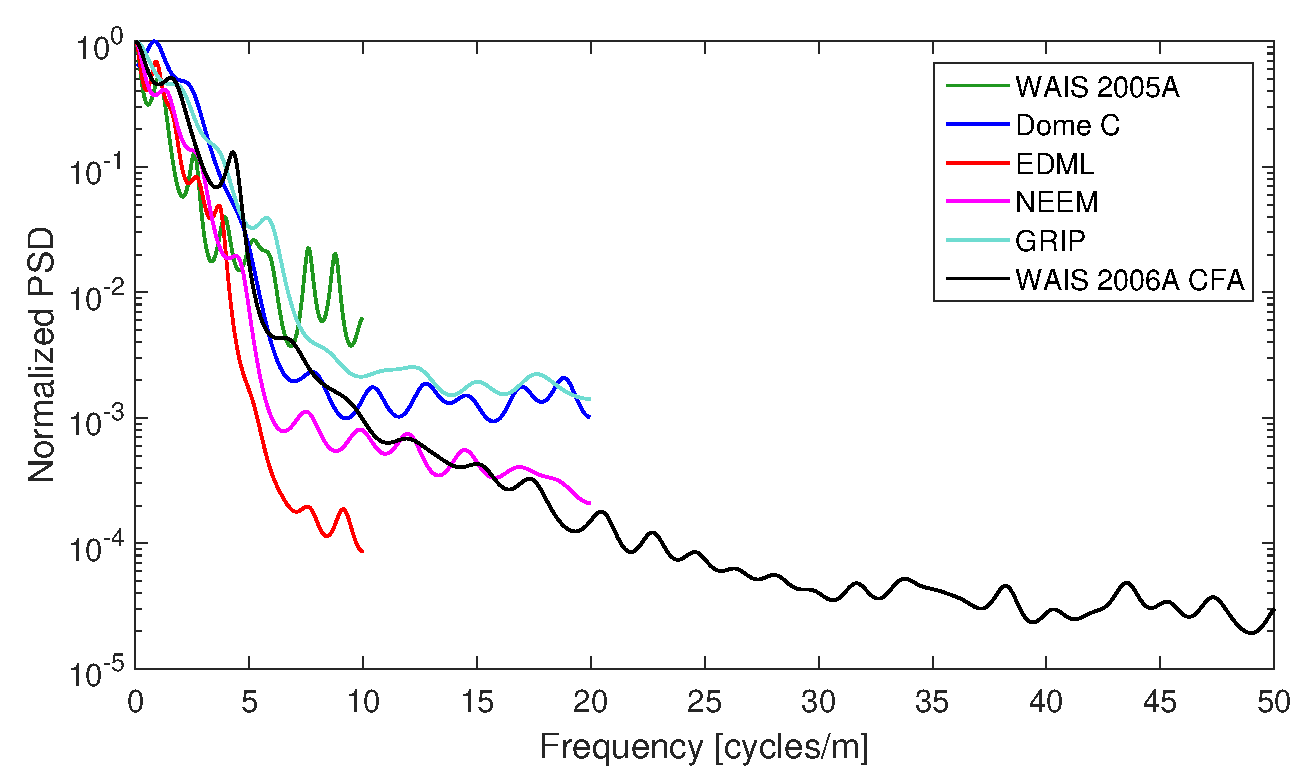
\includegraphics[width=0.9\linewidth]{PSD_discrete_plus_cfa_v1.eps}

	\end{minipage}%
	\begin{minipage}{0.5\textwidth}
		\centering
		\indent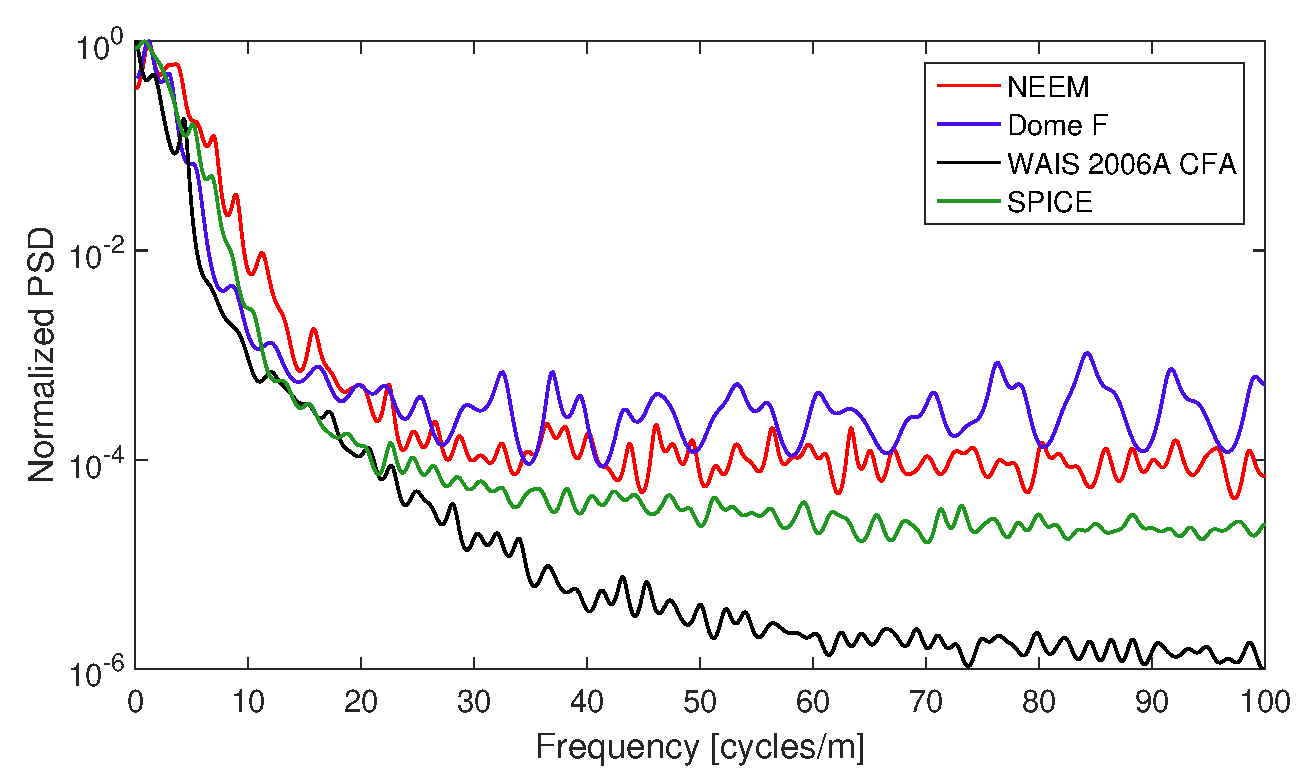
\includegraphics[width=0.9\linewidth]{PSD_CFA_v1.eps}

	\end{minipage}
	\caption{Left figure: The normalized PSD of five discretely measured $\delta^{18}$O series plotted together with the PSD of a $\delta^{18}$O WDC section. Right figure: The normalized PSD of four continuously measured $\delta$D series.}
\label{spectra_disVScfa}
\end{figure}

\begin{figure}
	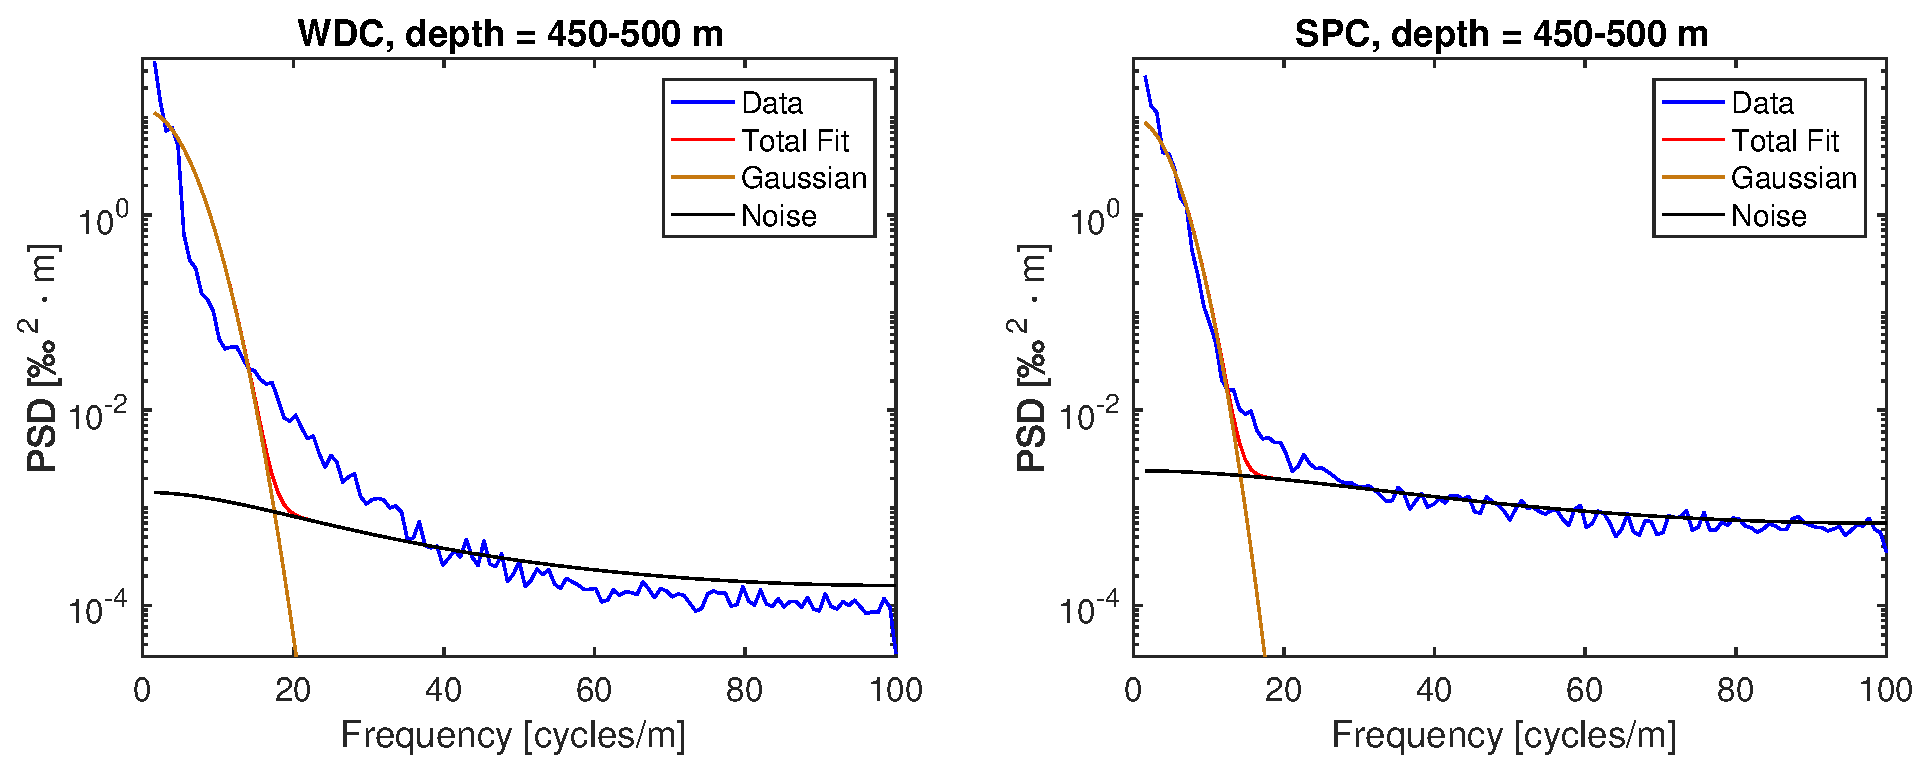
\includegraphics[width=\linewidth]{GR_fits.eps}
	\caption{Single-Gaussian multi-function fits for WDC and SPC at 450-500m depth.} \label{GR_fits}
\end{figure}

\begin{figure}
	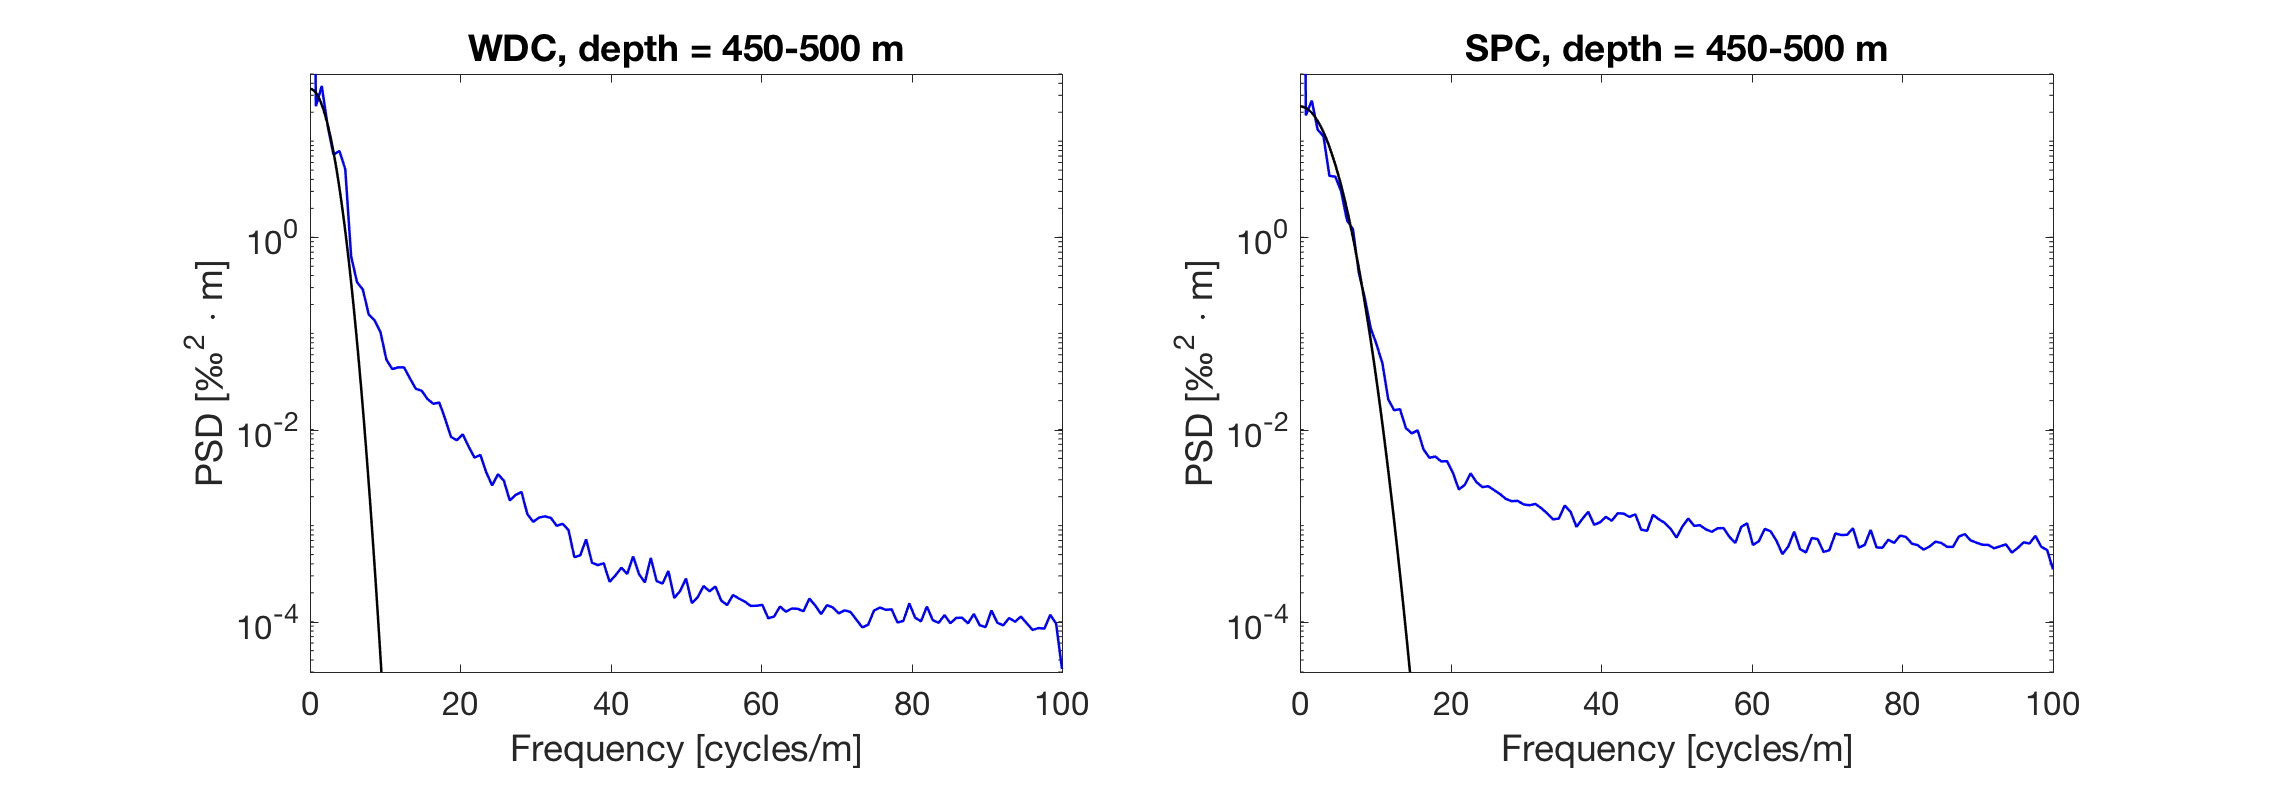
\includegraphics[width=\linewidth]{cutoff.eps}
	\caption{Cut-off technique on WDC and SPC at 450-500m depth. Blue curve is data spectrum and black curve is Gaussian fit.} \label{cutoff}
\end{figure}

\begin{figure}
	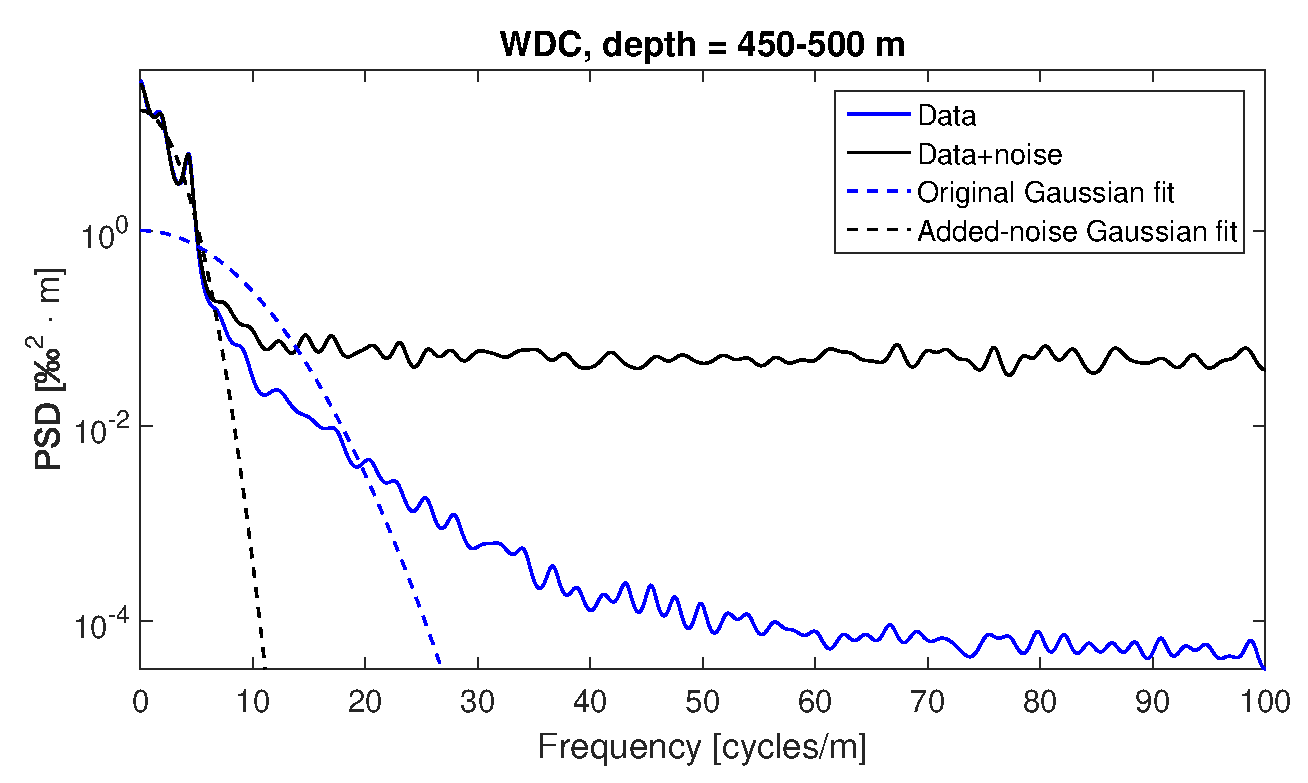
\includegraphics[width=.9\linewidth]{WAIS_spectrum_added_noise.eps}
	\caption{An illustration of the noise-adding technique for a $\delta$D section from WDC. The solid blue curve is the un-modified data and the black curve is data with noise added. The dashed lines represent the Gaussian functions fit using the two-function fitting technique.} \label{WAIS_spectrum_added_noise}
\end{figure}

\begin{figure}
	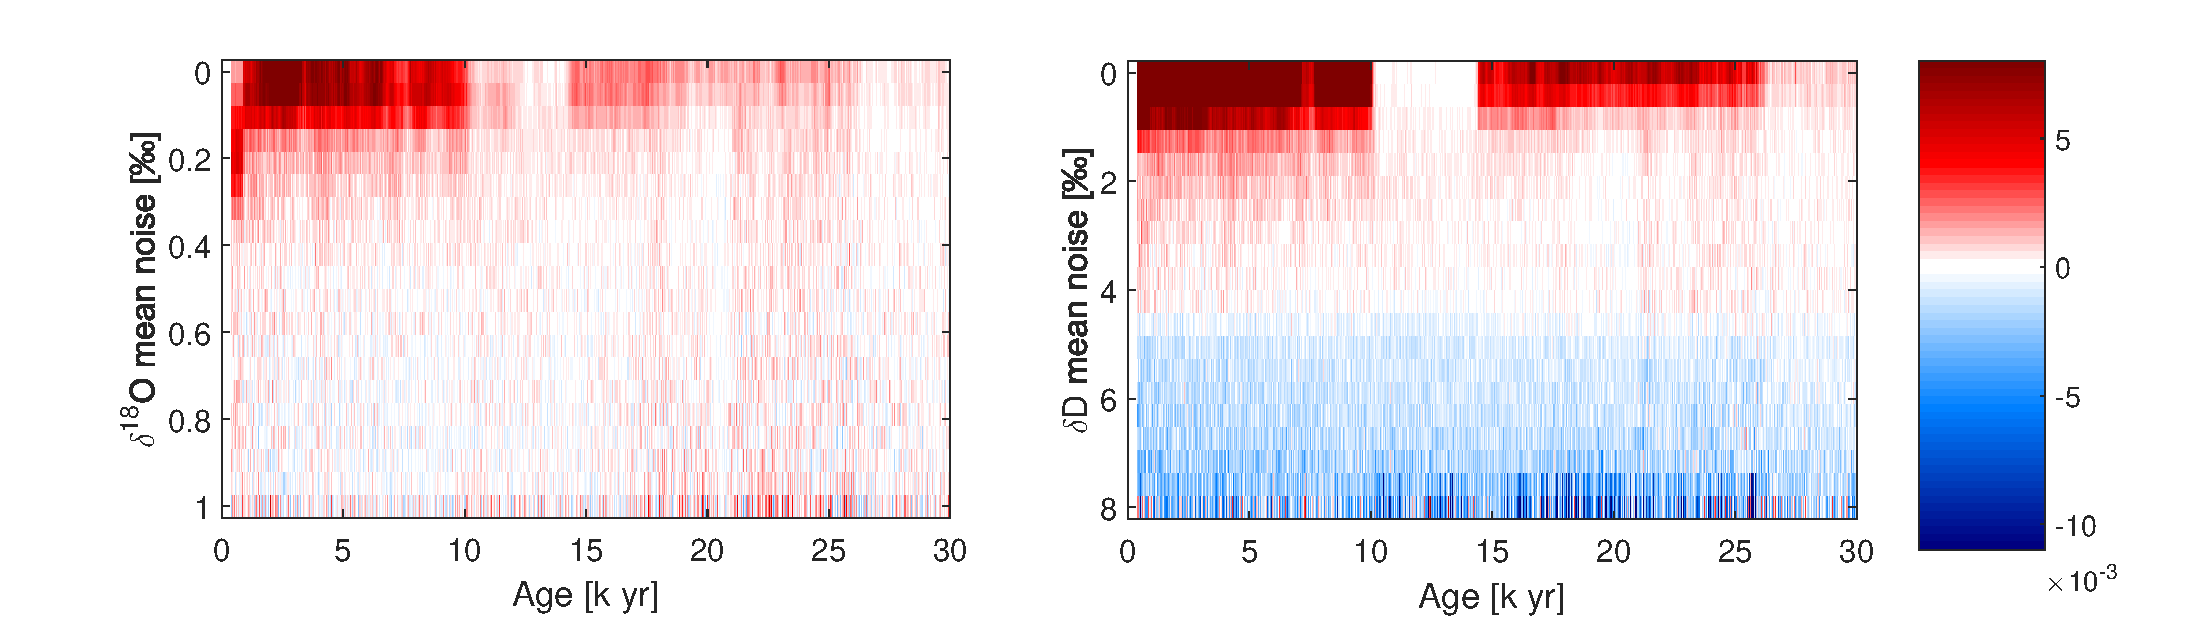
\includegraphics[width=\linewidth]{added_noise_sensitivity.eps}
	\caption{For WDC, the gradient of estimated diffusion lengths with respect to noise level plotted as a function of age. At each age, the lowest noise-level with a gradient of approximately zero is chosen as the optimal noise-level to be added.} \label{added_noise_sensitivity}
\end{figure}

\begin{figure}
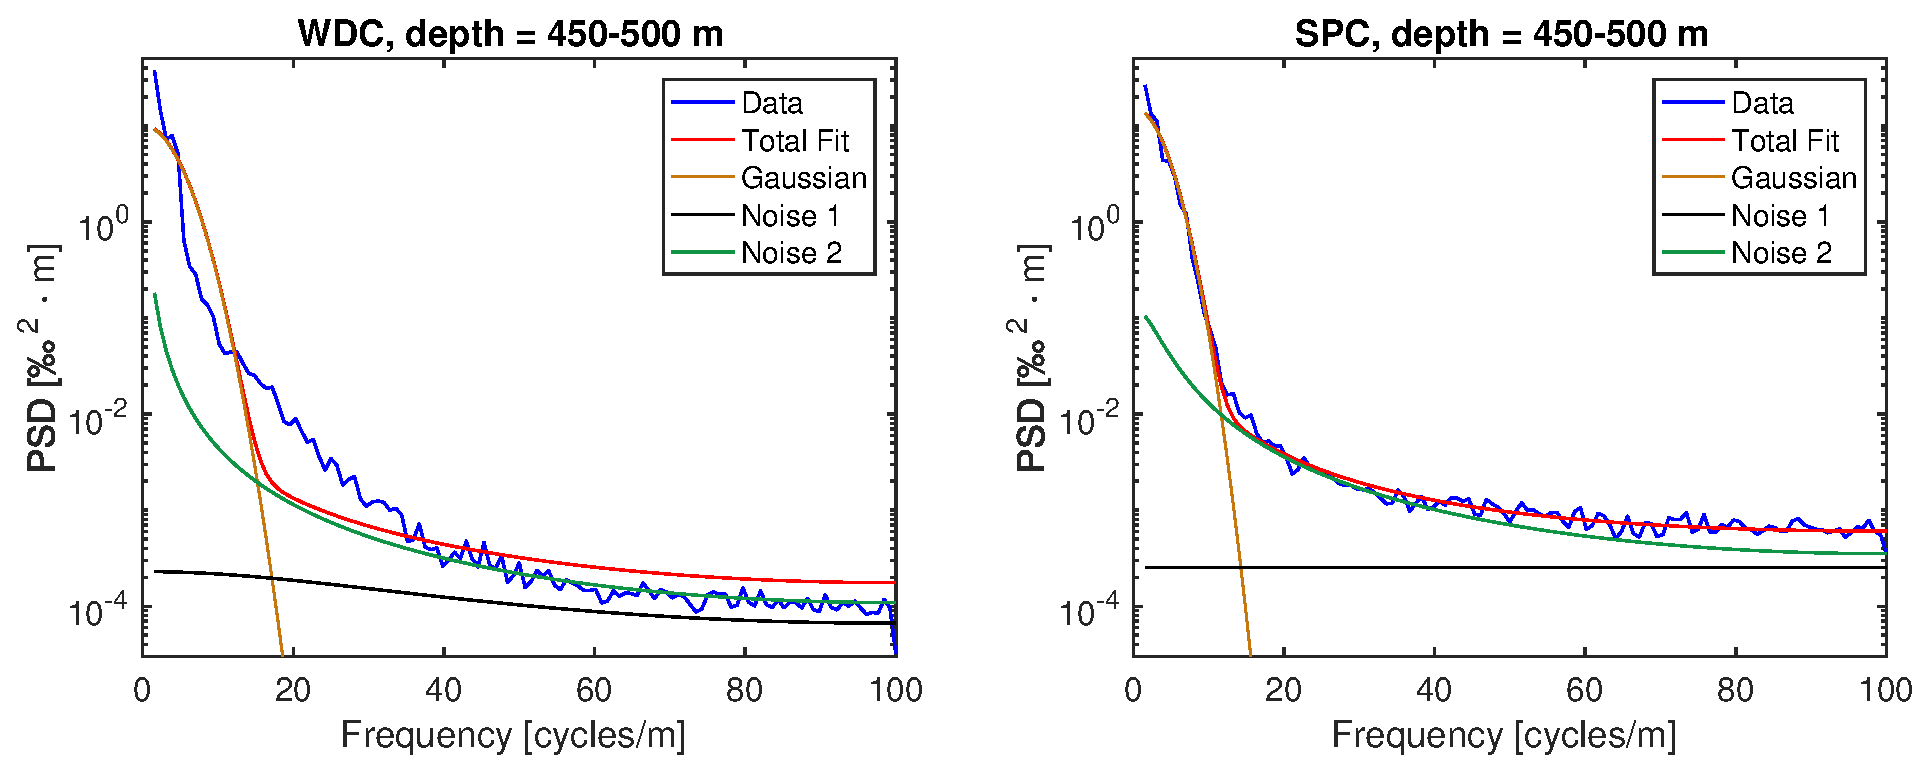
\includegraphics[width=.9\linewidth]{GRR_fits.eps}
\caption{Single Gaussian and two autoregressive-noise functions fit to WDC and SPC spectra.}\label{GRR_fits}
\end{figure}

\begin{figure}
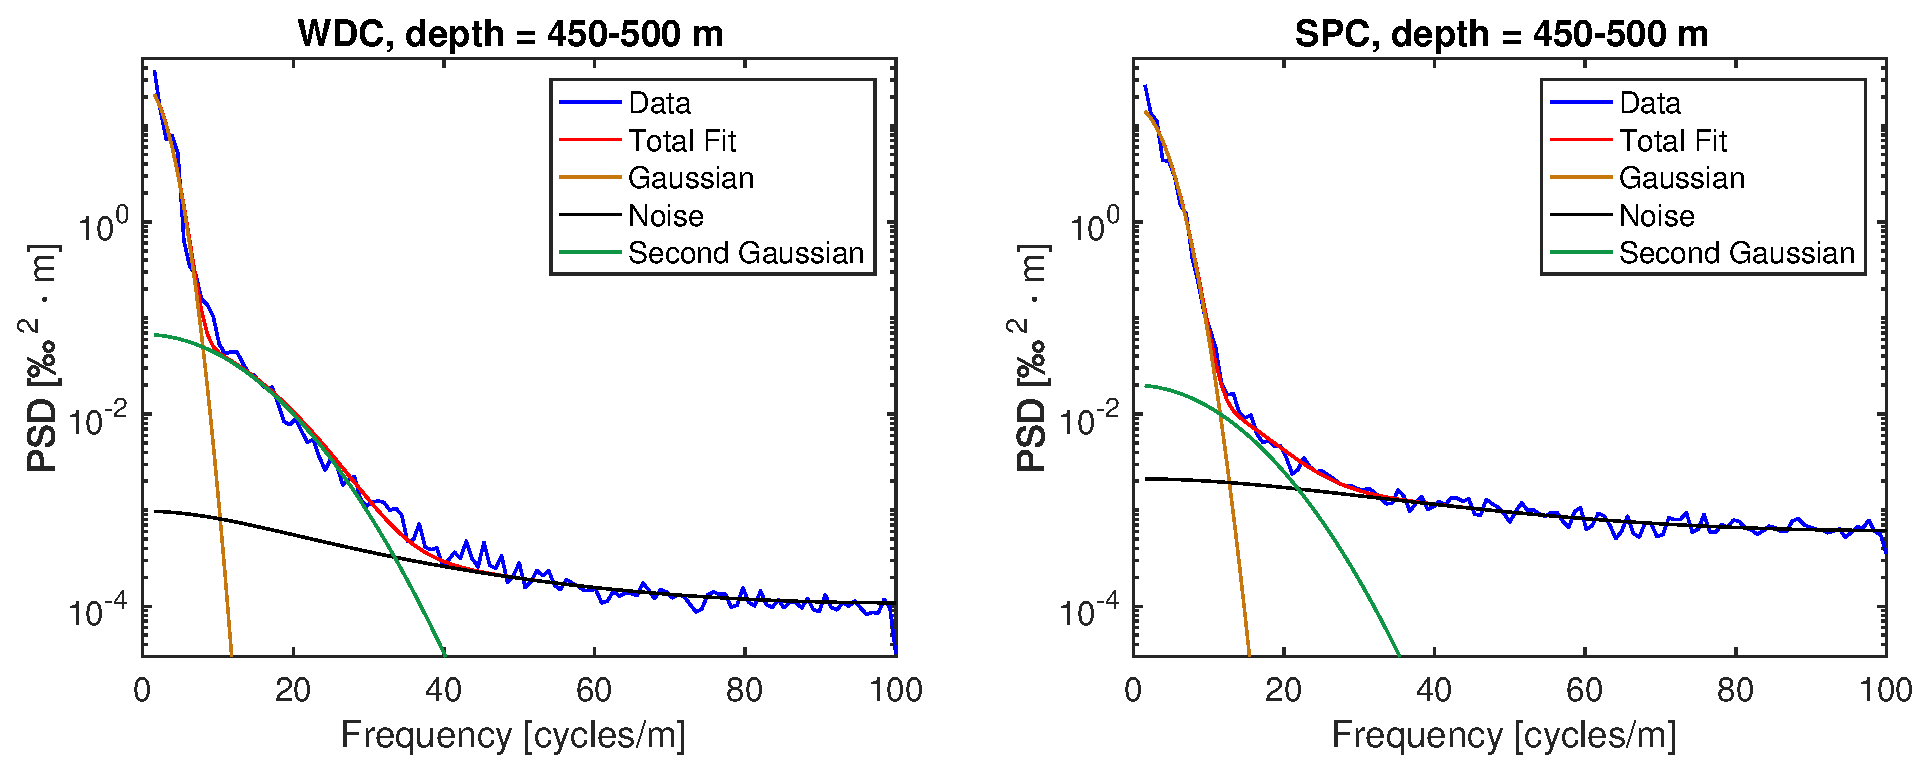
\includegraphics[width=.9\linewidth]{GGR_fits.eps}
\caption{Double-Gaussian multi-function technique fit to WDC and SPC spectra.}\label{GGR_fits}
\end{figure}

\begin{figure}
	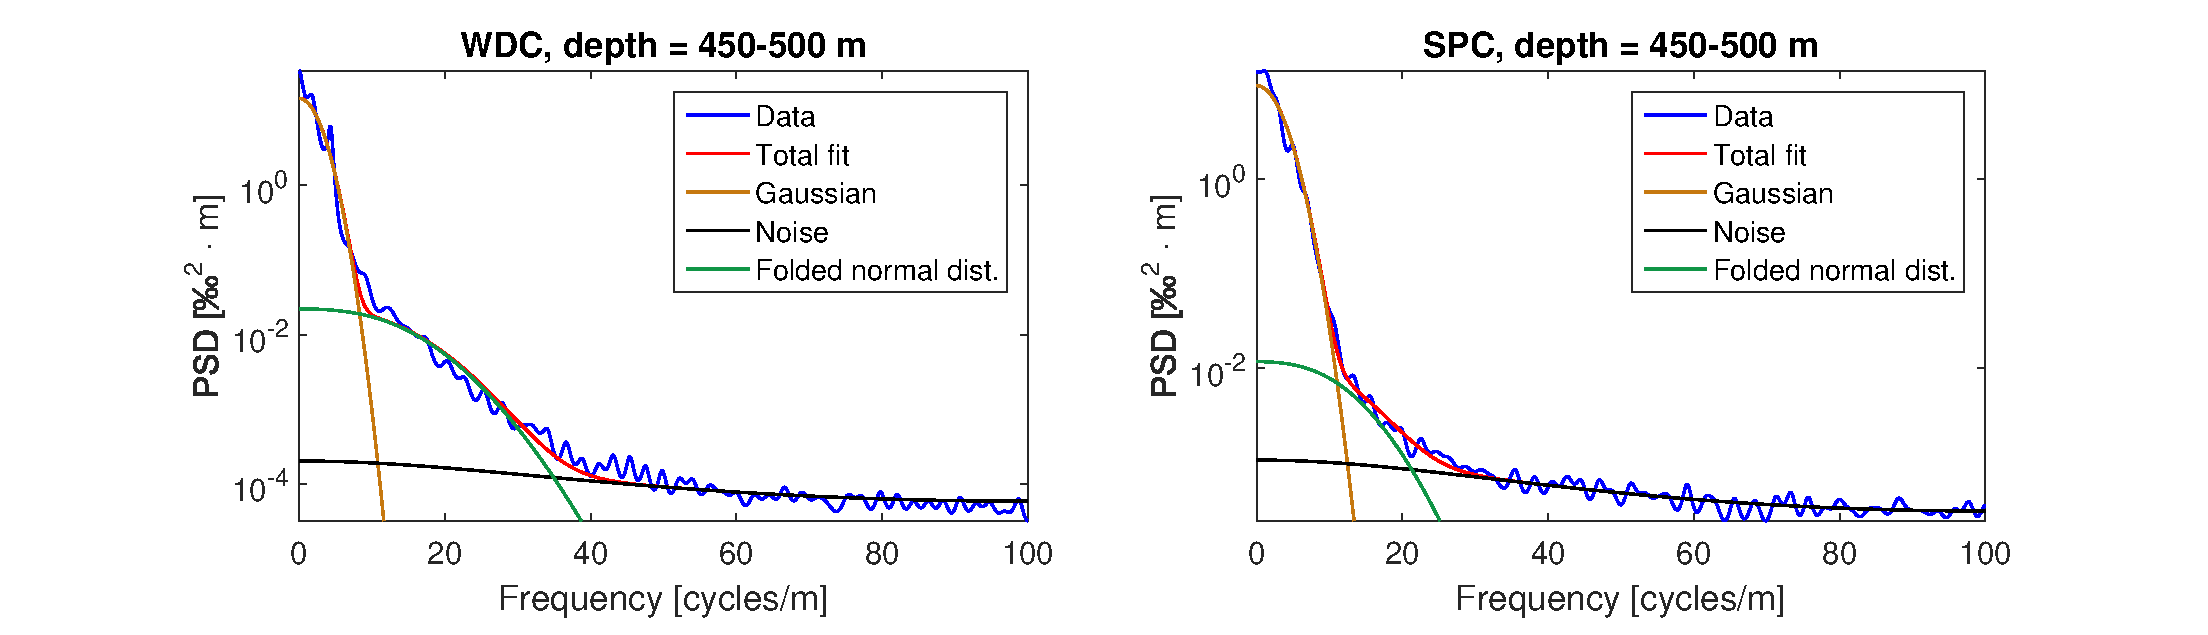
\includegraphics[width=1.1\linewidth]{folded_normal_gauss_spectrum.eps}
	\caption{Folded normal distribution multi-function technique fit to WDC and SPC spectra.}\label{folded_normal_gauss_spectrum}
\end{figure}

\begin{figure}
	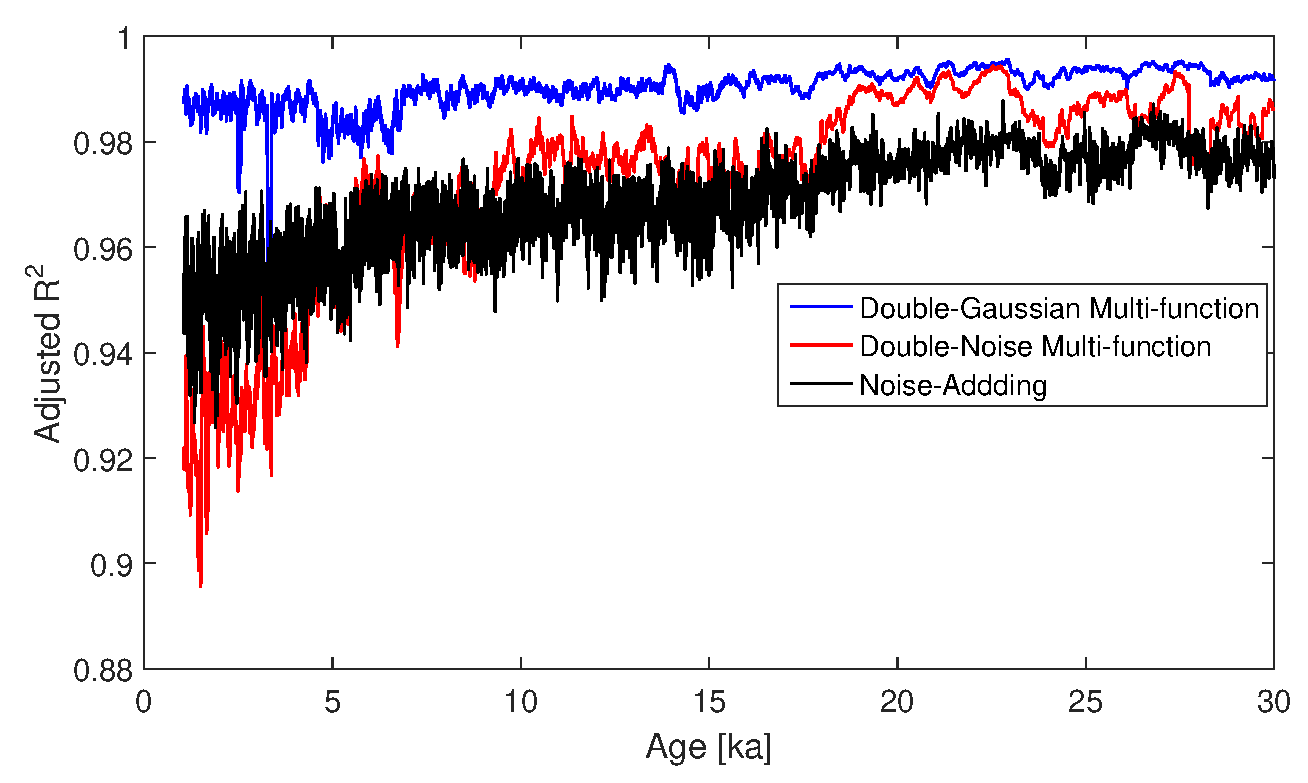
\includegraphics[width=.9\linewidth]{G_of_fit_1.eps}
	\caption{For WDC, the adjusted goodness of fit calculations through age for each fitting technique. FND results are identical to the results of a Gaussian curve and are not shown.} \label{G_of_fit_1}
\end{figure}

\begin{figure}
	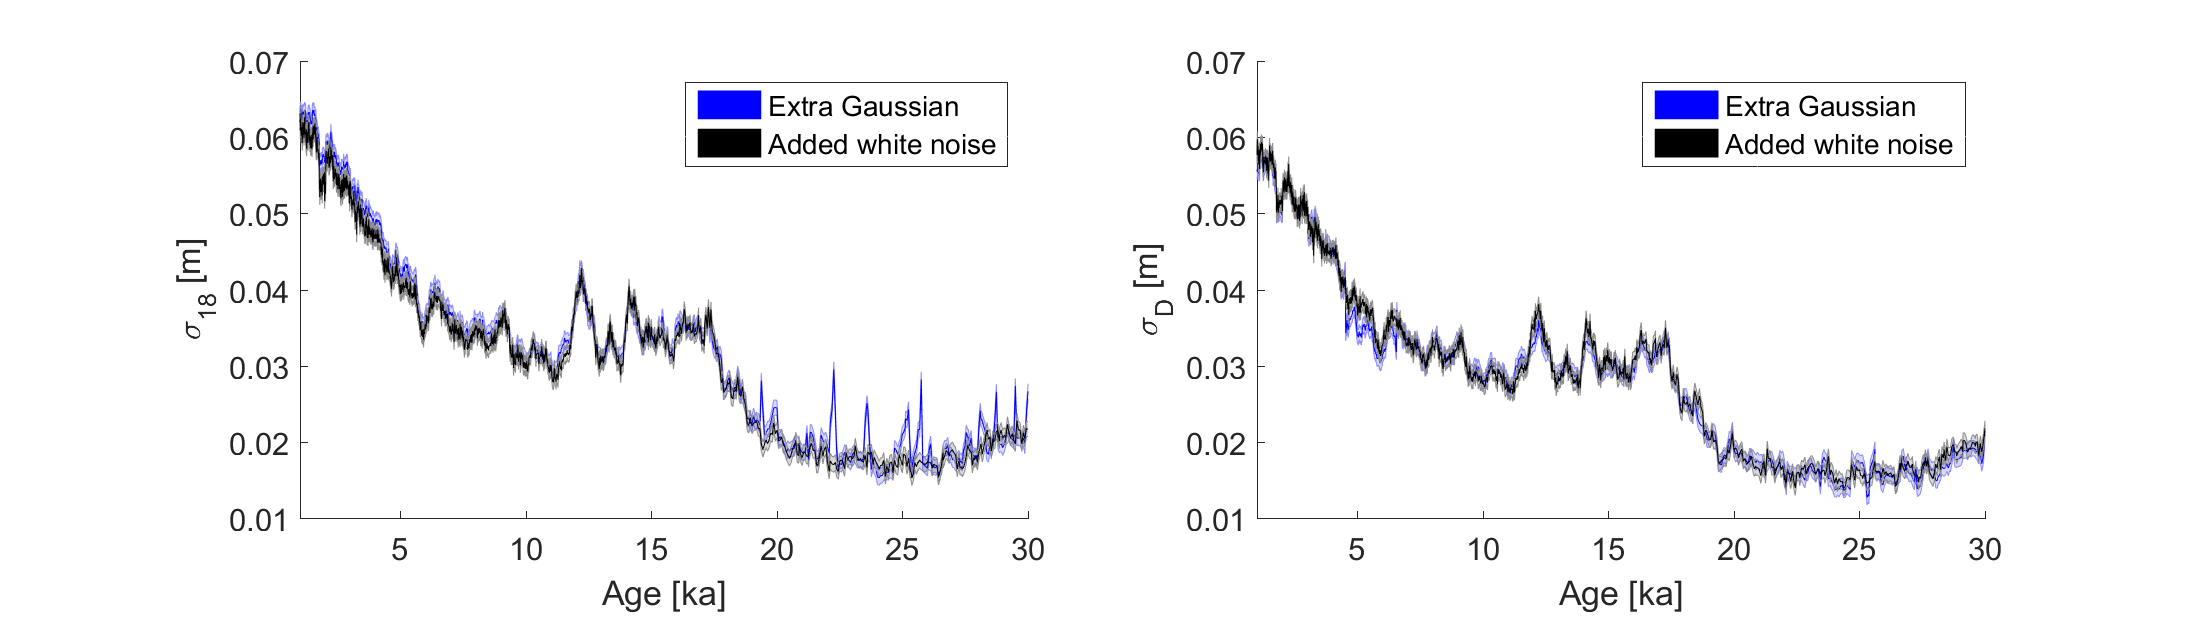
\includegraphics[width=\linewidth]{WAIS_diffusion_adding_noise.eps}
	\caption{WDC diffusion lengths of $\delta^{18}$O (left) and $\delta$D (right). Blue curve shows the multi-function Double-Gaussian technique, and the black curve shows the noise-adding technique.} \label{WAIS_diffusion_adding_noise}
\end{figure}

\begin{figure}
	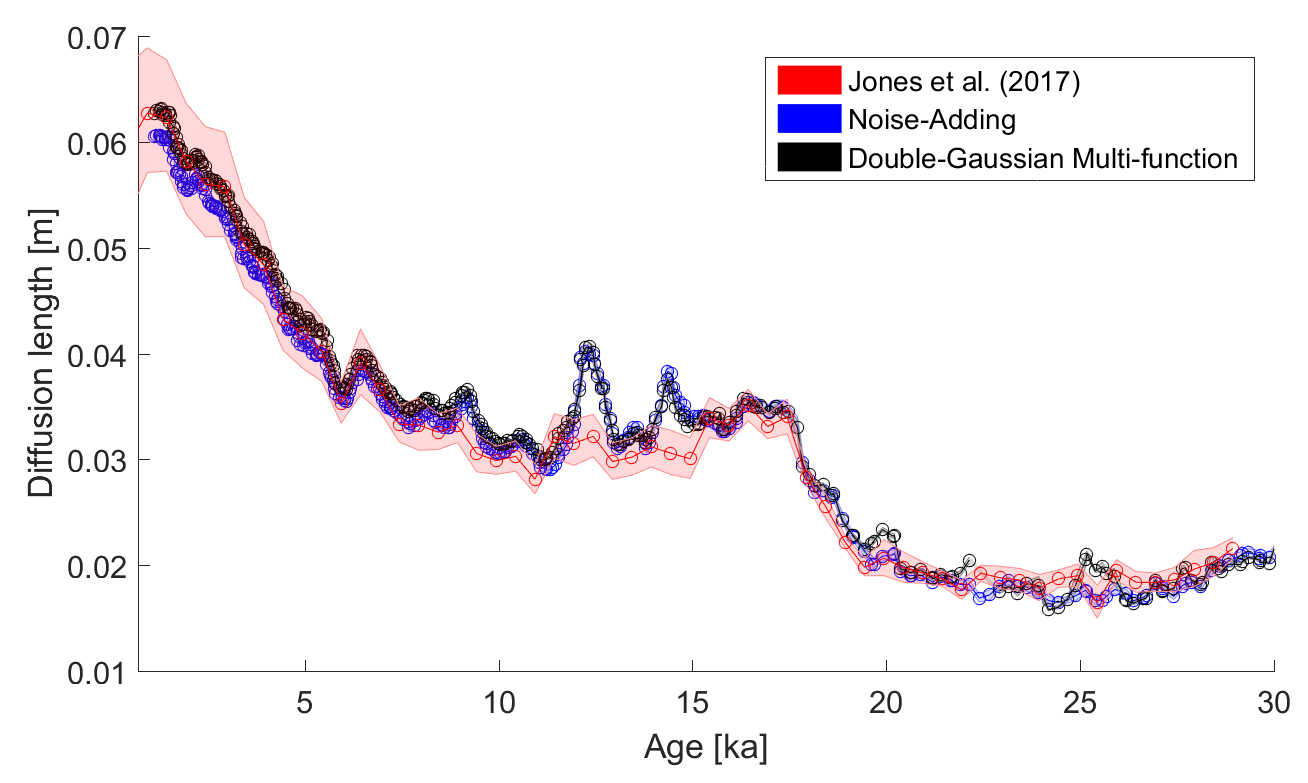
\includegraphics[width=.9\linewidth]{WAIS_diffusion_lengths.eps}
	\caption{Estimated WDC diffusion lengths of $\delta^{18}$O compared with those from \cite{Jones2017a}.} \label{WAIS_diffusion_lengths}
\end{figure}

\begin{figure}
	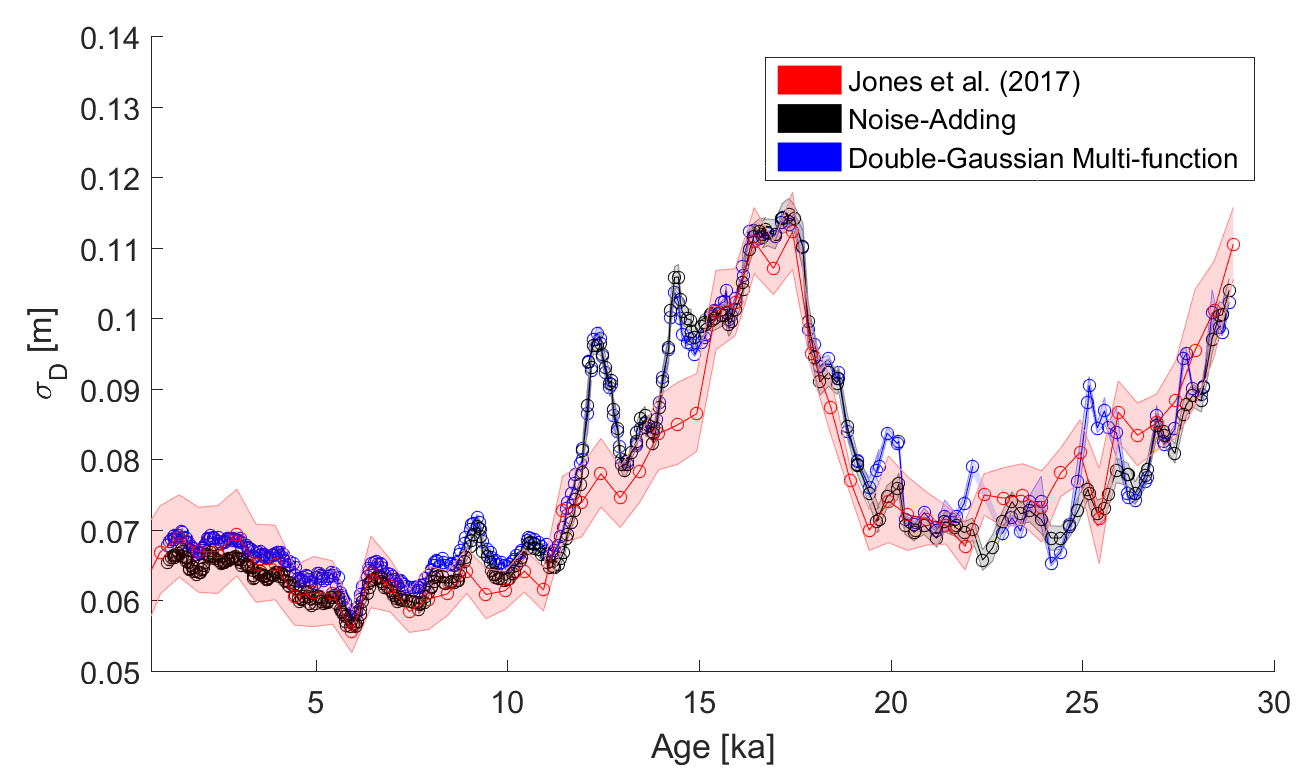
\includegraphics[width=.9\linewidth]{WAIS_diffusion_lengths_thinning_corr.eps}
	\caption{Thinning-corrected WDC diffusion lengths of $\delta^{18}$O compared with those from \cite{Jones2017a}.} \label{WAIS_diffusion_lengths_thinning_corr}
\end{figure}

\begin{table}
\caption{Temperature Estimates for SPC\tablenotemark{a}}\label{SP_deltaT}
\begin{tabular}{c|c c|c c c|c c}
\textbf{Technique} & \multicolumn{2}{|c|}{\textbf{6.7 - 7.5 ka}} & \multicolumn{3}{|c|}{\textbf{30.9 - 33.1 ka}} & \multicolumn{2}{|c}{\textbf{Temperature Difference}}\\
 & \textbf{$\delta$D} & \textbf{$\delta^{18}$O} & \textbf{$\delta$D} & \textbf{$\delta^{18}$O} & \textbf{$\delta^{17}$O} & \textbf{$\Delta$T $\delta$D} & \textbf{$\Delta$T $\delta^{18}$O}\\
\hline
Noise-adding & -56.7 & -54.3 & -61.8 & -58.4 & -56.8 & 5.1 & 4.1 \\
Double-Gaussian & -55.6 & -53.5 & -58.9 & -57.6 & -57.3 & 3.3 & 4.2 \\
\hline
mean & \multicolumn{2}{|c|}{-55.0} & \multicolumn{3}{|c|}{-58.5} & \multicolumn{2}{|c}{4.2} \\
standard deviation & \multicolumn{2}{|c|}{1.4} & \multicolumn{3}{|c|}{1.8} & \multicolumn{2}{|c}{0.7} \\
\end{tabular}
\tablenotetext{a}{Estimates made using 50-meter consecutive windows from 6.7 - 7.5 ka (450-500 meters) and 30.9-33.1 ka (1300 - 1350 meters). For each window, the noise-adding and double-Gaussian multi-function fitting techniques are used on on all available isotope data. The temperature difference between the two windows is also calculated. The means and standard deviations are given for each window, showing how well the techniques compare. All temperatures are in degrees C.}
\end{table}

\end{document}

%%%%%%%%%%%%%%%%%%%%%%%%%%%%%%%%%%%%%%%%%%%%%%%%%%%%%%%%%%%%%%%

More Information and Advice:

%% ------------------------------------------------------------------------ %%
%
%  SECTION HEADS
%
%% ------------------------------------------------------------------------ %%

% Capitalize the first letter of each word (except for
% prepositions, conjunctions, and articles that are
% three or fewer letters).

% AGU follows standard outline style; therefore, there cannot be a section 1 without
% a section 2, or a section 2.3.1 without a section 2.3.2.
% Please make sure your section numbers are balanced.
% ---------------
% Level 1 head
%
% Use the \section{} command to identify level 1 heads;
% type the appropriate head wording between the curly
% brackets, as shown below.
%
%An example:
%\section{Level 1 Head: Introduction}
%
% ---------------
% Level 2 head
%
% Use the \subsection{} command to identify level 2 heads.
%An example:
%\subsection{Level 2 Head}
%
% ---------------
% Level 3 head
%
% Use the \subsubsection{} command to identify level 3 heads
%An example:
%\subsubsection{Level 3 Head}
%
%---------------
% Level 4 head
%
% Use the \subsubsubsection{} command to identify level 3 heads
% An example:
%\subsubsubsection{Level 4 Head} An example.
%
%% ------------------------------------------------------------------------ %%
%
%  IN-TEXT LISTS
%
%% ------------------------------------------------------------------------ %%
%
% Do not use bulleted lists; enumerated lists are okay.
% \begin{enumerate}
% \item
% \item
% \item
% \end{enumerate}
%
%% ------------------------------------------------------------------------ %%
%
%  EQUATIONS
%
%% ------------------------------------------------------------------------ %%

% Single-line equations are centered.
% Equation arrays will appear left-aligned.

Math coded inside display math mode \[ ...\]
 will not be numbered, e.g.,:
 \[ x^2=y^2 + z^2\]

 Math coded inside \begin{equation} and \end{equation} will
 be automatically numbered, e.g.,:
 \begin{equation}
 x^2=y^2 + z^2
 \end{equation}

% IF YOU HAVE MULTI-LINE EQUATIONS, PLEASE
% BREAK THE EQUATIONS INTO TWO OR MORE LINES
% OF SINGLE COLUMN WIDTH (20 pc, 8.3 cm)
% using double backslashes (\\).

% To create multiline equations, use the
% \begin{eqnarray} and \end{eqnarray} environment
% as demonstrated below.
\begin{eqnarray}
  x_{1} & = & (x - x_{0}) \cos \Theta \nonumber \\
        && + (y - y_{0}) \sin \Theta  \nonumber \\
  y_{1} & = & -(x - x_{0}) \sin \Theta \nonumber \\
        && + (y - y_{0}) \cos \Theta.
\end{eqnarray}

%If you don't want an equation number, use the star form:
%\begin{eqnarray*}...\end{eqnarray*}

% Break each line at a sign of operation
% (+, -, etc.) if possible, with the sign of operation
% on the new line.

% Indent second and subsequent lines to align with the first character following the equal sign on the first line.

% Use an \hspace{} command to insert horizontal space into your equation if necessary. Place an appropriate unit of measure between the curly braces, e.g. \hspace{1in}; you may have to experiment to achieve the correct amount of space.


%% ------------------------------------------------------------------------ %%
%
%  EQUATION NUMBERING: COUNTER
%
%% ------------------------------------------------------------------------ %%

% You may change equation numbering by resetting
% the equation counter or by explicitly numbering
% an equation.

% To explicitly number an equation, type \eqnum{}
% (with the desired number between the brackets)
% after the \begin{equation} or \begin{eqnarray}
% command.  The \eqnum{} command will affect only
% the equation it appears with; LaTeX will number
% any equations appearing later in the manuscript
% according to the equation counter.
%

% If you have a multiline equation that needs only
% one equation number, use a \nonumber command in
% front of the double backslashes (\\) as shown in
% the multiline equation above.

%% ------------------------------------------------------------------------ %%
%
%  SIDEWAYS FIGURE AND TABLE EXAMPLES
%
%% ------------------------------------------------------------------------ %%
%
% For tables and figures, add \usepackage{rotating} to the paper and add the rotating.sty file to the folder.
% AGU prefers the use of {sidewaystable} over {landscapetable} as it causes fewer problems.
%
% \begin{sidewaysfigure}
% \includegraphics[width=20pc]{samplefigure.eps}
% \caption{caption here}
% \label{label_here}
% \end{sidewaysfigure}
%
% \begin{sidewaystable}
% \caption{}
% \begin{tabular}
% Table layout here.
% \end{tabular}
% \end{sidewaystable}
